\documentclass{article}
\usepackage[left=2.7cm, right=2.7cm, top=3cm]{geometry} % Change margins
\usepackage{mathtools} % falign
\usepackage{amsmath} % Basic maths
\usepackage{amssymb} % For some symbols
\usepackage{comment} % For comments
\usepackage{bm} % bold math
\usepackage{tikz} % For drawing trees
\usepackage{tikz-qtree} % For drawing trees
\usetikzlibrary{trees, positioning, arrows.meta, calc} % For drawing trees
\usepackage{xcolor} % Colouring equations
\usepackage{fancyhdr} % Cool headers
\usepackage{tabularx} % Fixed tables
\usepackage{graphicx}
\usepackage{multirow} % table merge row
\usepackage{color, colortbl} % colouring
\usepackage{tcolorbox} % for boxed stuffs, text + math mode
\usepackage{alltt} % better verbatim
\usepackage{wrapfig} % wrapping images with env wrapfigure
\usepackage[hidelinks]{hyperref}
\usepackage{booktabs} % better tables
\usepackage{float} % float tables
\usepackage[underline=false]{pgf-umlsd} % uml sequence diagrams
\restylefloat{table}
\usepackage{minted} % code highlighting
\usepackage{longtable} % tables that span multiple pages
\usepackage{enumitem} % \begin{enumerate}[label=(\alph*)]
\usepackage{pgfplots}
\usepackage{xifthen}% provides \isempty test
\usepackage{multirow}% multrow for table
\usepackage[font=small,labelfont=bf]{caption}

\usepackage{caption}
\usepackage{subcaption}

\def\BibTeX{{\rm B\kern-.05em{\sc i\kern-.025em b}\kern-.08em
    T\kern-.1667em\lower.7ex\hbox{E}\kern-.125emX}}

\pgfplotsset{compat=1.16} % Backwards compatibility

\usepackage{xargs} % Use more than one optional parameter in a new commands

\usepackage[sorting=none]{biblatex}
\addbibresource{refs.bib}

% A really nice TODO package and helpers
% https://tex.stackexchange.com/questions/9796/how-to-add-todo-notes
\setlength {\marginparwidth }{2cm}
\usepackage[colorinlistoftodos,prependcaption,textsize=tiny]{todonotes}
\newcommandx{\todoany}[2][1=]{\todo[inline,#1]{[\sectionlabel{}]~#2}}
\newcommandx{\todojim}[2][1=]{\todo[linecolor=red,backgroundcolor=red!25,bordercolor=red,inline,#1]{[\sectionlabel{}]~\textbf{Jim}:~#2}}
\newcommandx{\tododuke}[2][1=]{\todo[linecolor=blue,backgroundcolor=blue!25,bordercolor=blue,inline,#1]{[\sectionlabel{}]~\textbf{Duke}:~#2}}
\newcommandx{\gtododuke}[2][1=]{\todo[linecolor=blue,backgroundcolor=blue!25,bordercolor=blue,#1]{[\sectionlabel{}]~\textbf{Duke}:~#2}}
\newcommandx{\tododhruv}[2][1=]{\todo[linecolor=green,backgroundcolor=green!25,bordercolor=green,inline,#1]{[\sectionlabel{}]~\textbf{Dhruv}:~#2}}
\newcommandx{\gtododhruv}[2][1=]{\todo[linecolor=blue,backgroundcolor=blue!25,bordercolor=blue,#1]{[\sectionlabel{}]~\textbf{Dhruv}:~#2}}

\hypersetup{
  colorlinks=true,
  urlcolor=blue,
  linkcolor=black,
  citecolor=black
}

% circled numbers
\newcommand*\circled[1]{\tikz[baseline = (char.base)]{%
            \node[shape=circle,draw,inner sep=2pt] (char) {#1};}}%

% For use in align*
\newcommand*\mathcomment[1]{&&{#1}}
\newcommand*\mathcommentt[1]{&&{\text{#1}}}

\usepackage{amsthm} % For Proofs
\newtheorem*{remark}{Remark}
\renewcommand\qedsymbol{}

\begin{document}

\pagestyle{fancy}
\fancyhf{}
\lhead{COMP9491: Project Report}
\rhead{Duck News Reporters}
\cfoot[C]{\thepage}

% L{3cm} for a ragged right paragraph in tabular tables.
\newcolumntype{L}[1]{>{\raggedright\let\newline\\\arraybackslash\hspace{0pt}}m{#1}}

\renewcommand{\headrulewidth}{1pt}
\renewcommand{\footrulewidth}{0.5pt}

\newcommand{\sectiontitle}{}
\newcommand{\subsectiontitle}{}
\newcommand{\sectionlabel}{\ifdefempty{\subsectiontitle}{\sectiontitle}{\sectiontitle/\subsectiontitle}}
\newcommand{\newsection}[1]{\section{#1}\renewcommand{\sectiontitle}{#1}\renewcommand{\subsectiontitle}{}}
\newcommand{\newsubsection}[1]{\subsection{#1}\renewcommand{\subsectiontitle}{#1}}

% \begin{noindent}
\newcommand{\articlecontent}[1]{%
	\ifthenelse{\equal{#1}{118real}}{FBI Director James Comey said Sunday that
	the bureau won't change the conclusion it made in July after it examined
	newly revealed emails related to the Hillary Clinton probe.

	``Based on our review, we have not changed our conclusions that we
	expressed in July with respect to Secretary Clinton'' Comey wrote in a
	letter to 16 members of Congress. [...]
	}{}%
  \ifthenelse{\equal{#1}{1fake}}{Hillary in hot water over her email server,
  again. Sacramento, CA — Democratic nominee Hillary Clinton is in hot water
  again after nearly 5 million uncounted California electronic ballots were
  found on her email server by the F.B.I. The majority of those ballots cast
  were by Bernie Sanders supporters. [...] }{}%
  \ifthenelse{\equal{#1}{128real}}{[...]I have a prediction. I know exactly what
  November 9 will bring. Another day of God’s perfect sovereignty.

  He will still be in charge. His throne will still be occupied. He will still
  manage the affairs of the world. Never before has His providence depended on a
  king, president, or ruler. And it won’t on November 9, 2016. “The LORD can
  control a king’s mind as he controls a river; he can direct it as he pleases”
  (Proverbs 21:1 NCV).
  
  On one occasion the Lord turned the heart of the King of Assyria so that he
	aided them in the construction of the Temple.  On another occasion, he stirred
	the heart of Cyrus to release the Jews to return to Jerusalem. [...]}{}%
  \ifthenelse{\equal{#1}{2fake}}{Washington, D.C. – South African Billionaire,
  Femi Adenugame, has released a statement offering to help African-Americans
  leave the United States if Donald Trump is elected president. According to
  reports, he is offering \$1 Million, a home and car to every Black family who
  wants to come to South Africa.

  Concerns about Donald Trump becoming president has prompted a South African
  billionaire to invest his fortune in helping African-Americans leave the
  United States to avoid further discrimination and inequality. [...]}{}%
  \ifthenelse{\equal{#1}{10fake}}{The Internet is buzzing today after white
  supremacist presidential candidate Donald Trump was caught by hotel staff
  snorting cocaine.

  Maria Gonzalez an employee at the Folks INN \& Suites Hotel in Phoenix brought
  room service to his room witnessed it all.
  
  ``When I walked in I saw 3 naked prostitutes and maybe 100,000 in hundred
  dollars bills and a mountain of white powder on the table, I thought it was a
  dog on the floor sleep but it was his hair piece, he was bald and sweating
  like crazy.'' [...]}{}%
	\ifthenelse{\equal{#1}{15fake}}{After hearing about 200 Marines left
	stranded after returning home from Operation Desert Storm back in 1991,
	Donald J.Trump came to the aid of those Marines by sending one of his planes
	to Camp Lejuene, North Carolina to transport them back home to their
	families in Miami, Florida.

	Corporal Ryan Stickney was amongst the group that was stuck in North
	Carolina and could not make their way back to their homes. [...]
	}{}%
  \ifthenelse{\equal{#1}{34fake}}{It has been more than fifteen years since Rage
  Against The Machine have released new music. The members of the band have
  involved themselves in various other projects during their lengthy hiatus, but
  one pressing issue has forced the band to team up once again.

  In a statement posted online, Rage Against The Machine announced they would be
	releasing a brand new album aimed at spreading awareness about ``how awful
	Donald Trump is''. [...]
	}{}%
}
\newcommand{\articletitle}[1]{%
	\ifthenelse{\equal{#1}{118real}}{FBI Completes Review of Newly Revealed Hillary Clinton Emails Finds No Evidence of Criminality}{}%
  \ifthenelse{\equal{#1}{1fake}}{5 Million Uncounted Sanders Ballots Found On Clinton's Email Server}{}%
}
% \end{noindent}

\title{\textbf{Duck News Reporters: Automated fake news detection through contextual similarity comparison}\\\vspace*{12pt}\large{COMP9491: Applied Artificial Intelligence --- Project Report}}
\author{%
  Dhruv Agrawal\\
  \texttt{z5361800@unsw.edu.au}
  \and
  Duke Nguyen\\
  \texttt{z5398432@unsw.edu.au}
  \and
  Jim Tang\\
  \texttt{z5208565@unsw.edu.au}
}

\maketitle
\thispagestyle{empty}

\listoftodos % DELETE THIS BEFORE SUBMIT

\newsection{Introduction}

\todoany{Describe the problem domain and aim of study, briefly introduce the developed methods and summarise your experimental findings}

As the distribution of news shifts towards social media, there is a rise in the dissemination of fake news. We define fake news as the creation of information presented as legitimate journalism that describes a fictitious event or fabricates details of an event in an attempt to mislead readers. This phenomenon became a major focal point in journalism during the 2016 US elections with political parties labelling many publications and articles as fake news. There are two huge issues with how this occurred in 2016:

\begin{enumerate}
  \item Many prominent political figures highlighted any news they disagreed with as fake news. This led to the political isolation of the party, whereby any news that looked at them unfavourably had the potential to be dismissed as fake news This reduced the accountability of political figures in the US, a country where federal legislation has a sweeping impact across the country and the rest of the world.
  \item There was a lack of fake news detection tools on social media and due to the polarisation of the media climate, it was extremely difficult for social media to regulate articles published on the platforms or remove factually incorrect articles posted or shared by politicians.
\end{enumerate}

Since then, there have been many attempts to introduce ways to deal with these issues such as Politifact which manually reviews articles and social media posts for factual correctness. It posts its findings on its website and is easily accessible for people. Other similar websites exist but the reason manual fact-checking tools are not as prominent in spaces with high amounts of fake news is because it is impossible for manual review tools to scale to the number of news articles and journalistic social media posts published every day.

There are also many automated fake news detection algorithms which rely on linguistic features of the text, comparisons between the title of the article and its content, the medium of transmission, and any suspicious activity linked with its engagement online. These tools have become more effective since COVID and Twitter employs its own automated algorithms to automatically label articles about certain topics it chooses as fake news. However, these tools are known to be very unreliable as it is increasingly common for fake news to read the same way as real news articles and be shared by humans.

Therefore, in order for fake news detection to become more widespread and effective in combating fake news, there are a few different criteria it must fulfil:

\begin{enumerate}
  \item The algorithms need to automatically classify news as real or fake so that they can scale with the growth of social media and the increase in fake news dissemination.
  \item The algorithms need to incorporate current methods of fake news detection as these have been highly researched and are effective in many situations such as when fake news has been automatically generated or constructed in a highly polarised manner designed to provoke intense responses from readers.
  \item An additional feature that looks at the content and meaning of the article beyond how has been written must be used to combat fake news that is well-written and designed to look like real news.
  \item The dataset used to train and assess the algorithms must contain real and fake articles that are written in the same style so that it is not apparent simply from the way an article is written whether it is real or fake.
\end{enumerate}

Our approach improves upon existing approaches and aims to combine the above criteria to analyse both the content and style of articles and make a significantly more informed decision on its classification. The model is restricted to a binary classification - it outputs either real or fake rather than giving a confidence metric of an article's legitimacy. This is done as the aim is for the tool be easily adopted and focusing on the simplicity of the input and output is a priority.

We compiled a list of commonly used linguistic features for fake news detection. Multiple different pairings of features were formed and analysis was conducted to determine the most effective linguistic features for the task. This takes existing research into fake news detection and puts our model in line with current methods. A new feature - similarity - is used to achieve the third criterion above. At a high level, this feature compares the queried article to other articles on Google news which are at the top of Google's searches. As these have high PageRank scores, the model can be confident that they are real articles and it compares the similarity of the content between the queries article and each of these top searched articles. This is done as a way for the model to infer context before making a judgement on an article's legitimacy. This approach brings out model in line with the way humans manually fact-check articles which usually involves finding known trustworthy sources and comparing the content between the articles to determine whether the queried one is consistent with the trustworthy ones.

Through this research, we have analysed and determined the most effective linguistic features for fake news detection and shown that the use of similarity as a metric is effective in building upon these current metrics to increase accuracy. We have also compared the use of the similarity metric with different machine learning classifiers and discovered that it greatly increases the accuracy of less complex machine learning methods and brings their performance in line with complex models.

\newsection{Related work}

\tododhruv{Describe the current state-of-the-art or related literature in this problem domain}

\newsection{Methods}

\begin{minipage}{\textwidth}
  \begin{wrapfigure}{r}{0.65\textwidth}
    \vspace*{-20pt}
    \centering
    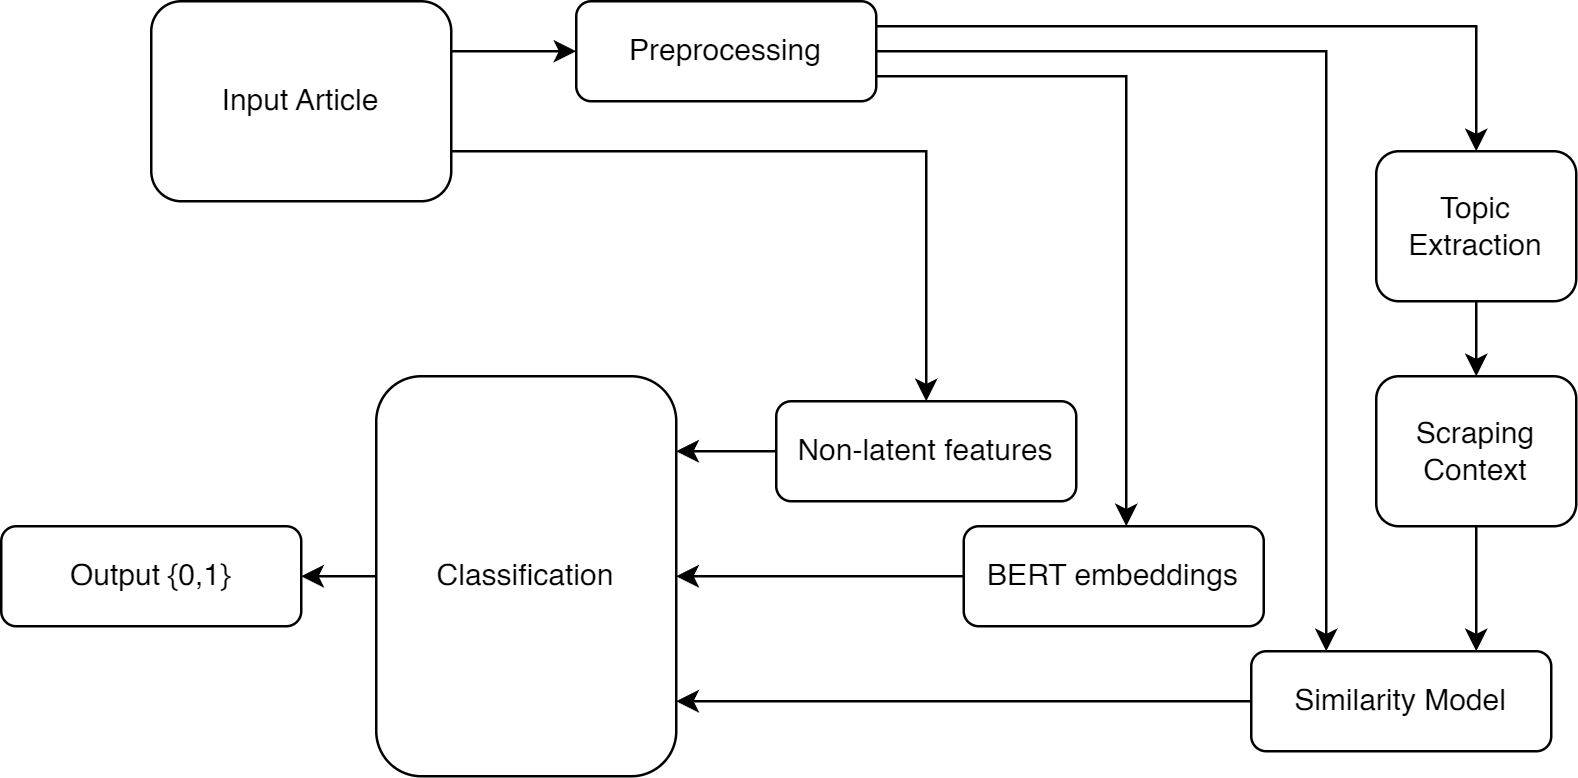
\includegraphics[width=0.6\textwidth]{img/pipeline.png}
    \caption{Our classification pipeline.}
    \label{pipeline}
  \end{wrapfigure}

  Figure~\ref{pipeline} shows our mostly linear classification pipeline. After preprocessing and tokenization, we extract contextual articles which are fed into a similarity model to form our first feature. Additionally, non-latent features from raw text and BERT embeddings form the rest of our features. The concatenation of all the features are fed into our classification models which infers a binary classification label.
\end{minipage}

\newsubsection{Preprocessing and tokenization}\label{section:preprocessing}

Before extracting any features, we will preprocess our input and convert the long form text into tokens. We perform the following preprocessing methods in order:

\begin{quote}
  \textbf{Remove non-ascii:}\quad Our input articles contained unnecessary unicode tokens such as unicode double quotation marks. These can be removed safely since they do not add any extra semantics to the input articles and may confuse feature extraction.

  \textbf{Convert to lowercase:}\quad In our research, we converted all text to lowercase. However upon further analysis, converting all text to lowercase hid acronyms such as ``US'' which could have affected the main themes of the text. Further, all proper nouns such as names and places were also hidden. We will discuss this limitation in Section~\ref{limitation:preprocessing}.

  \textbf{Lemmatization:}\quad We used the \verb|nltk|~\cite{nltk} libaray to reduce words down to their lemma in the hopes of reducing the complexity within our text which may benefit feature extraction. This looks up the work in the WordNet corpus to get the lemma. Later in the research, we realised that this hypothesis may have not been accurate.

  Firstly the \verb|nltk| library we were using does not automatically detect the part of speech and will by default, only lemmatize nouns. While it is arguably better for us to maintain the tense of nouns, we are technically not lemmatizing fully. Secondly, from more research, lemmatization may not be ideal for BERT embeddings since it removes some semantics that could be learnt by the BERT model. We will discuss these limitations further in Section~\ref{limitation:preprocessing}.

  \textbf{Remove stopwords:}\quad Stopwords were removed from the text in order to reduce complexity.
\end{quote}

Apart from the above methods, we also tested removing punctuation. However, this was not used in the end since we added non-latent features to measure punctuation counts and also to maintain semantics for BERT.

After preprocessing, tokens are then generated based on any whitespace and punctuation in the remaining text. Table~\ref{preprocessing} shows samples of tokenized input articles.

\begin{table}
  \begin{center}
    \makebox[0pt]{\begin{minipage}{\paperwidth}
        \centering
        \subfloat{
          \begin{tabular}{cp{8cm}p{6cm}}
            \toprule
            ID & Article extract & Tokens\\
            \midrule
            118\_Real & \small{\articlecontent{118real}}
            & \small{['fbi', 'director', 'james', 'comey', 'said', 'sunday', 'bureau', 'change', 'conclusion', 'made', 'july', 'examined', 'newly', 'revealed', 'email', 'related', 'hillary', 'clinton', 'probe', '.', '"', 'based', 'review', ',', 'changed', 'conclusion', 'expressed', 'july', 'respect', 'secretary', 'clinton',\ldots]}\\
            \midrule
            15\_Fake & \small{\articlecontent{15fake}}
            & \small{['hearing', '200', 'marines', 'left', 'stranded', 'returning', 'home', 'operation', 'desert', 'storm', 'back', '1991', ',', 'donald', 'j', '.', 'trump', 'came', 'aid', 'marines', 'sending', 'one', 'plane', 'camp', 'lejuene', ',', 'north', 'carolina', 'transport', 'back', 'home', 'family', 'miami',\ldots]}\\
            \bottomrule
          \end{tabular}
        }
        \hfill
      \end{minipage}}
  \end{center}
  \caption{Examples of preprocessing and tokenization extraction on items in dataset.}
  \label{preprocessing}
\end{table}

\newsubsection{Feature --- BERT embeddings}
BERT (Bidirectional Encoder Representations from Transformers) is a language representation model proposed by Devlin et al \cite{bert}. It is pretrained on BookCorpus and the English Wikipedia using masked language modeling (MLM) and next sentence prediction (NSP). MLM masks some of the input tokens with a training objective to predict the masked token simply based on context, and the model also concatenates two sentences with 50\% chance of being neighbouring sentences, and the model is pre-trained in the NSP layer to predict if the two are indeed neighbours \cite{bert}. BERT obtains SOTA results on several tasks and is suitable for representing document and textual data. Hence, we will be using BERT as the main feature to encode our articles. We will use HuggingFace's 'bert-base-uncased' pretrained model which trains on uncased data. To encode an article, we slice the first 512 tokens of the respective article and pass it through 'bert-base-uncased' and output the CLS token's vector as BERT features for our classification model.

\newsubsection{Feature --- Non-latent features} \label{section:non-latent-feat}

\begin{figure}[h]
  \centering
  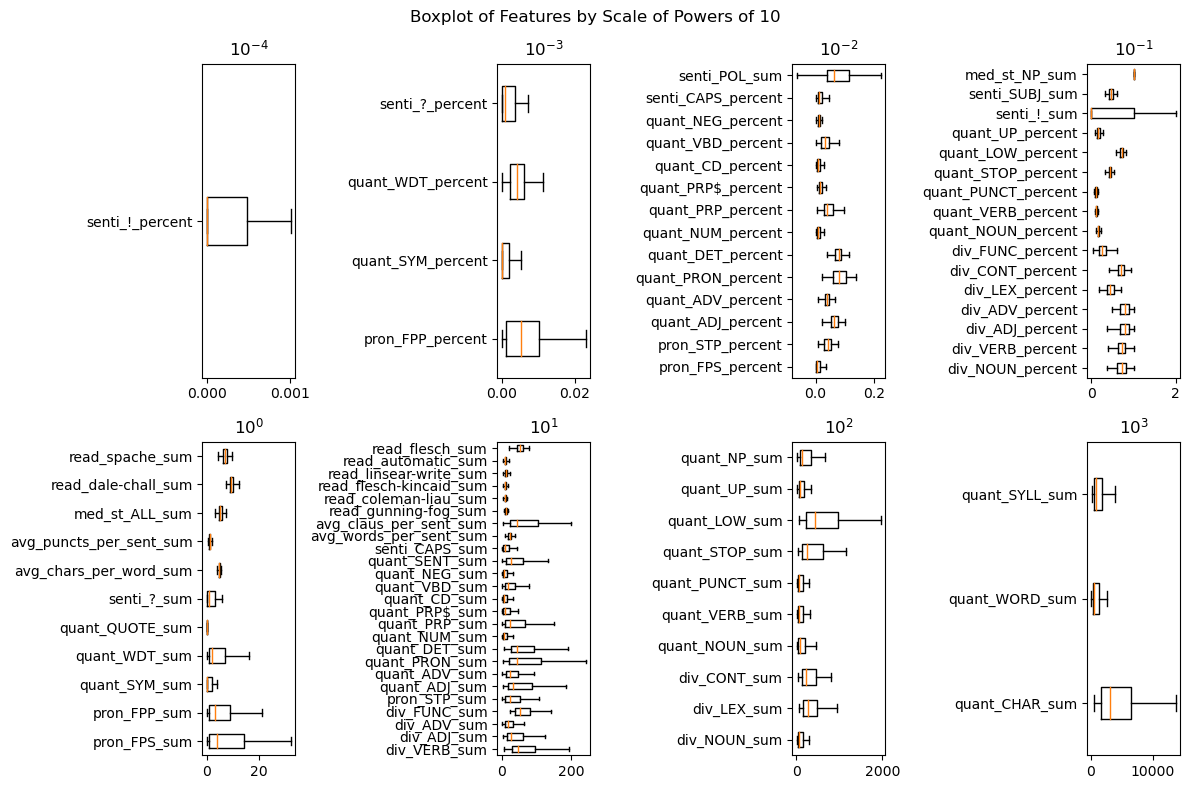
\includegraphics[width=\textwidth]{img/non_latent_box_plot.png}
  \caption{Non Latent Box Plot Features}
  \label{box-plot}
\end{figure}

From our literature review and survey, we are able to identify a significant amount of non-latent features \cite{zhou2020survey, garg2022linguistic, horne2017}. After combining features that are similar, and removing features which we cannot calculate due to the need for proprietary softwares (i.e. LIWC), or due to the computational complexity of the algorithms, or related reasons, we are able to identify 81 numerical features suitable for our experiments. After synthesising their categorisations in the original articles, we come up with a grouping of 7 main categories (with their abbreviation in brackets), with each feature being able to calculated with a few methods:
\begin{itemize}
  \item Diversity (div): number of unique words, or percentage of all unique words of a particular part of speech (e.g. noun, verb)
  \item Quantity (quant): number of words, or percentage of all words of a particular part of speech or linguistic unit (e.g. noun, adjective, quote)
  \item Sentiment (senti): number of linguistic features denoting sentiment (e.g. exclamation mark, all-cap words), or sentiment measurement (polarity, subjectivity)
  \item Pronoun (pron): number of pronouns of a specific class (e.g. first person singular pronoun: I, me, my, mine)
  \item Average (avg): average number of linguistic unit \texttt{a} per linguistic unit \texttt{b} (e.g. characters per word)
  \item (Median) Syntax Tree Depth (med\_st): the median syntax tree depth of a given unit (e.g. median noun phrase syntax tree depth)
  \item Readability (read): different readability indices (e.g. gunning-fog, coleman-liau)
\end{itemize}

The feature names are designated using the format "\texttt{category}\_\texttt{featureType}\_\texttt{calculationMethod}", where category is the abbreviated \texttt{category}, \texttt{featureType} is the feature type within the category. Appendix \ref{appendix:non-latent-table} contains a full description and explanation of all non-latent features, their category, feature type, and their calculation method. Figure \ref{box-plot} is a box plot of all the non-latent features by their scale of power of 10. The majority of features are between the range of $[10^{-2}, 10^{1}]$. Several quantity and some diversity features are in the higher range of $[10^2, 10^3]$.

\begin{figure}[h]
  \centering
  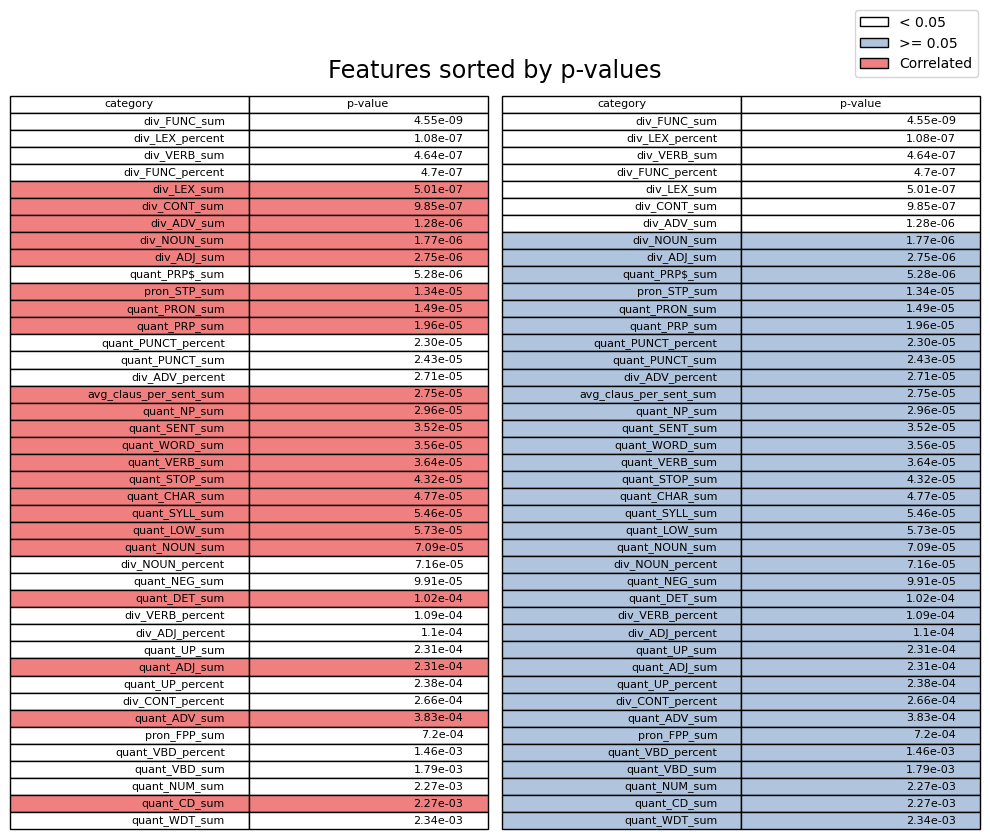
\includegraphics[width=\textwidth]{img/non_latent_feat_prune.png}
  \caption{Non-Latent Feature Pruning}
  \label{fig:non-latent-feat-prune}
\end{figure}

We can then apply ANOVA on these non-latent features against the labels, and filter for those with a p-value less than the $\alpha$ significance level of 0.05. We identify that the removed features account to almost half of all features, and they include readability indices, the syntax tree depth features, and a few features from other categories, and diversity features are all below $\alpha$. We then apply Pearson correlation amongst the selected features and identify all correlation clusters. The matrix is available in Appendix \ref{appendix:correlation-matrx}. Afterwards, we can apply a selection method on the cluster where we remove all but one with the lowest p-value, specifically, we sort the selected features by p-value in ascending order with the lowest p at the front of the list, we then search for all features which have a correlation of at least $0.95$ and remove them from the current list, and continue until the end. Figure \ref{fig:non-latent-feat-prune} shows our results. After grouping them by their original category, we have the following counts, totalling to 29 features, which we will use for our classification models:
\begin{itemize}
  \item Diversity: 9 features
  \item Quantity: 12 features
  \item Pronoun: 2 features
  \item Sentiment: 3 features
  \item Average: 1 feature
\end{itemize}

\newsubsection{Feature --- Similarity model}

\tododuke{Explain the point of similarity model: Hypothesis - we hypothesize that articles that are real vs false are more dissimilar than articles that are both real. We assume context articles are real}
As a novel feature, we investigate the similarity of our input articles to contextual articles found online. In Sections~\ref{section:summary-extraction} and~\ref{section:article-scraping} we will discuss our process of gathering three contextual articles from online sources which we treat as truth. These are then vectorized and fed into a similarity model which we describe in Sections~\ref{section:similarity-metric} and~\ref{section:similarity-metric}. We use this similarity as a feature to ascertain whether our input article contains misinformation.

\subsubsection{Summary extraction} \label{section:summary-extraction}

To get the context articles, we need to summarize the main topic of our input article down to at most 10 keywords. We use the Python \verb|gensim|~\cite{py-gensim} library which provides various topic modelling interfaces for text inputs. We use the \verb|ldamodel| which implements Latent Dirichlet Allocation (LDA) to extract a single topic. LDA is a probabilistic model where the idea is you have a number of documents representing some latent topics characterized by a distribution over words. By feeding in the preprocessed sentences of our input article, we are able to get the main themes. We sort the output keywords by the probability they represent the topic then cap the amount of words to 10 at most.

For the scope of our research, we are able to perform manual validation of the summaries extracted to check the summary represented the article content well. Table~\ref{summary-extraction} shows some samples of items in our dataset after applying LDA. We see that while the summaries extracted are not perfect, they still represent the general meaning of the article. Two common issues we saw were:
\begin{itemize}
  \item Unordered words in the summary --- words representing the topics seemed to be unordered. To a human reading the summary by itself, they might be able to see that the words are all keywords of the article but put together in a sentence, will not completely make sense. We hypothesize that this could have caused sub-optimal results when we started scraping articles using the summaries.
  \item Appearance of stop words and other meaningless non-topic words in the summary --- As a flow on issue from our preprocessing, our summary was left with words such as ``wa'' (from ``was'') or ``ha'' (from ``has''). This would have impacted the meaning of our summary and later article scraping.\label{summary-extraction:bad-words}
\end{itemize}
We will discuss the possibility of extracting better summaries using a more robust model in Section~\ref{limitation:summary-extraction}.

\begin{table}
  \centering
  \begin{tabular}{cp{8cm}p{3cm}}
    \toprule
    ID & Article extract & Summary\\
    \midrule
    118\_Real & \small{\articlecontent{118real}}
    & email review fbi clinton said july comey news new wa\\
    \midrule
    15\_Fake & \small{\articlecontent{15fake}}
    & home marines trump wa stickney way north plane family\\
    \bottomrule
  \end{tabular}
  \caption{Examples of summary extraction on items in dataset.}
  \label{summary-extraction}
\end{table}

\subsubsection{Article scraping} \label{section:article-scraping}

We feed the summary of the input article into Google News and collect the top three articles. We use Google News since it essentially provides a free PageRank algorithm which we can leverage to get the most popular articles during the time period. We will treat the articles we find as Real articles for purposes of comparison, i.e.\ an input article that is very different to our contextual article is likely to be Fake.

For our research, we will only manually feed in all summaries for our dataset. Our motivation for this research was to develop a tool that a user could potentially use to figure out if the current news they are reading contains misinformation. We acknowledge there exists APIs that provide either a wrapper around Google News or implement their own news search algorithm that we could have looked into. However, given the size of the dataset and our scope, this was not necessary to demonstrate our system.

\begin{quote}
  \textbf{SETUP:} We use a virtual machine with a freshly installed latest version of Google Chrome. Searches are condicted in ``Incognito Mode'' tabs. We also use a VPN to the West coast of the US. These invariants serve the main purpose so that Google's does not give any personalized results based on a browser fingerprint or IP address. We chose the US as the VPN destination since our dataset articles were extracted from US news sources and we wanted to scrape for articles with a similar style of writing. If you were to use the tool in Australia, Google would usually return articles from local sources. We restrict our scope to specifically this dataset rather than train on a wide dataset from all sources.

  Another invariant we implement is to add a \verb|before:2020| to our summary. This forces Google News to only find articles before this year so that the news we get won't be from recent news. A common discussion topic from our dataset was Donald Trump's 2016 election campaign and we know that the news regarding Trump in 2023 is much different to that of 2016. This makes sense as we are not using a very recent dataset so clamping the date we find contextual articles assumes that if were looking for fake articles at the time of reading the imput article, we wouldn't have too much future articles available.

  \textbf{PROCESS:} We attempt to get the top three articles and save the URL for each input article. Not all summaries returned three articles so we perform scraping in three passes:
  \begin{enumerate}
    \item We enter the whole summary without any changes. This is the most ideal approach and most machine-replicable. This covered 70\% of our dataset.
    \item Still performing only generic actions, we remove any~\hyperref[summary-extraction:bad-words]{\color{blue}bad words} or non-important connectives then searched again. This should still be machine-replicable with further work. This covered the next 20\% of our dataset.
    \item For the last 10\% of our dataset, we had to manually look at the input article content and summary generated to figure out why we still received no results. Our hypothesis was that this was a combination of our non-tuned summary extraction and the fact that some \emph{outrageous} Fake articles simply didn't have any similar articles that could be found. We will discuss this limitation in Section~\ref{limitation:article-scraping}.
  \end{enumerate}
  From the above passes, we were not able to find context articles for four input articles described in a table in Appendix~\ref{appendix:article-scraping}. Furthermore, we were only able to find one or two articles for some inputs but we can still continue with our similarity model.
\end{quote}

\begin{figure}[H]
  \centering
  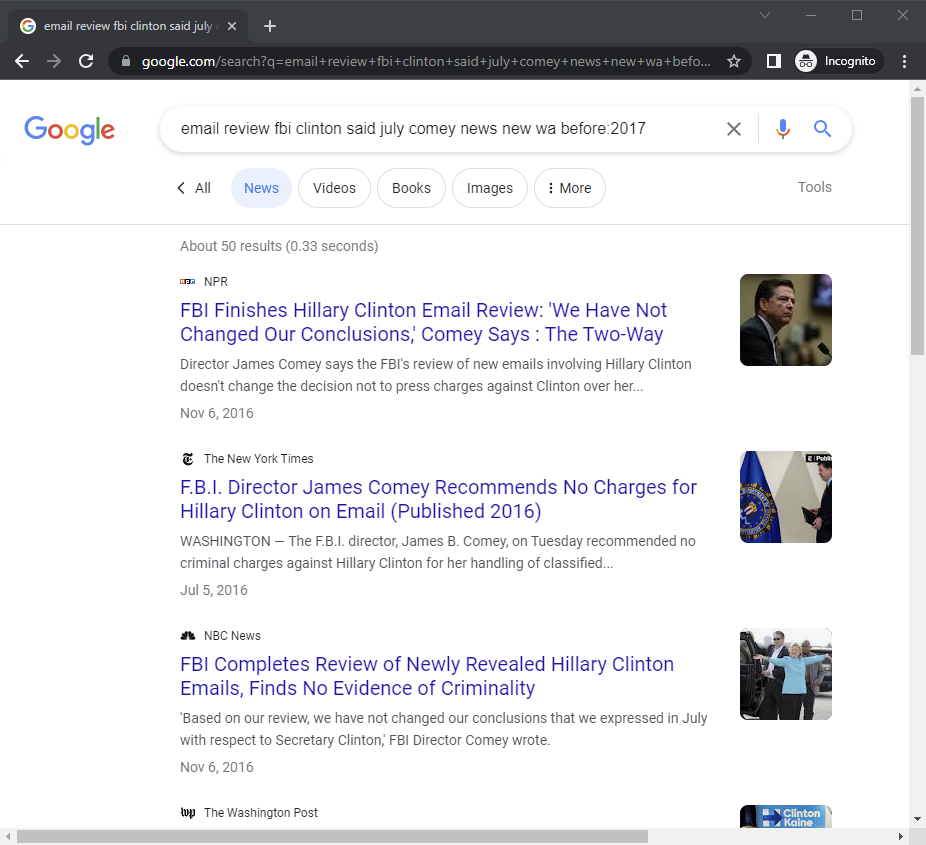
\includegraphics[width=0.4\textwidth]{img/chrome-article-scraping.png}
  \caption{Sample of articles found in Google after searching an article summary.}
\end{figure}

\noindent
After gathering three URL links for each context article, we use the Python \verb|newspaper3k|~\cite{py-newspaper} library to download the article and automatically extract its title and content.

% \subsubsection*{Similarity model}
% Once we have context articles for each input article, we can apply a transformation on the two to obtain their vector representations (a process called article vectorisation), after which we can apply a metric on the two article vectors and output a numeric value representing the similarity between the two corresponding articles (a process which we call similarity metric calculation). We will now discuss different approaches to article vectorisation and similarity metric calculation.

\subsubsection{Article vectorisation} \label{section:article-vectorisation}
\tododuke{Cite one more article here that also does the same similarity metric calculation}
Past research by Alsuliman, et. al in~\cite{alsuliman2022social} proposes two different ways to vectorise the articles: TF-IDF, and Word2Vec. In addition to these two vectorisation methods, we propose a third -- \emph{``non-latent vectoriser''}.

\begin{quote}
  % https://scikit-learn.org/stable/modules/generated/sklearn.feature_extraction.text.TfidfTransformer.html#:~:text=The%20formula%20that%20is%20used,document%20frequency%20of%20t%3B%20the
  \textbf{TF-IDF~\cite{scikit-learn}:}\quad The term frequency times inverse document frequency, which is a \emph{``common term weighting scheme in information retrieval''}. The formula given as follows:

  \[\frac{article.count(term)}{len(article)} * \log_2{\left(\frac{len(articles)}{df(articles, term)} + 1\right)}\]

  The first term is the term frequency, and the second term is the inverse document frequency, where \texttt{article} is the article we are applying TF-IDF on, \texttt{article.count(term)} is the frequency of \texttt{term} in \texttt{article}, \texttt{len(article)} is the number of words in the article, \texttt{len(articles)} is the number of articles, \texttt{df(articles, term)} is the document frequency of \texttt{term} in our \texttt{articles} dataset, or the number of articles that contains this term  \cite{scikit-learn}. The formula given has a '+1' term in idf so that the algorithm would not ignore terms that appear in all articles, this is the \texttt{sklearn} implementation and differs from the standard textbook formula which has the '+1' in the denominator in log2 of idf  \cite{scikit-learn}. TF-IDF will be fitted on the original dataset of input articles (for \texttt{articles} in IDF term), then be used as vectorize to transform both the input and context articles. We will apply TF-IDF in two n-gram ranges of (1,1) and (1,2).

  % gensim, alsuliman2022social
  % https://radimrehurek.com/gensim/models/word2vec.html
  % https://code.google.com/archive/p/word2vec/
  \tododuke{Cite Alsuliman or the article that pioneered the use of document vec as the average vec in this case}
  \textbf{Word2Vec~\cite{word2vec-google}:}\quad A word embedding architecture introduced by Google in 2013. It uses continous bag-of-words (CBOW), which uses neighbouring words to predict target words, and continuous skip-gram which uses target words to predict the neighbouring words, using either hierarchical softmax or negative sampling \cite{gensim} \cite{mikolov2013efficient}. We will be using the gensim implementation of word2vec using the pretrained 'word2vec-google-news-300' model which is trained on the Google News dataset of about 100 billion words containing 3 million words and phrases in 300 dimensions. We chose this model due to the similarity between the domain of its dataset and out dataset being news. To calculate the article vector, we retrieve the vector of every single word in an article, existing those that do not exist in the embeddings, and then taking the average from the list \cite{alsuliman2022social}.

  \textbf{Non-Latent Vectorizer:}\quad The non-latent vectorizer uses the non-latent feature selected in Section \ref{section:non-latent-feat} and apply them on an article into a vector. This is the non-latent vector presentation of the respective article.
\end{quote}


\subsubsection{Similarity metric calculation} \label{section:similarity-metric}

Past research by Alsuliman et al. in~\cite{alsuliman2022social} proposes three different metrics to calculate the similarity between two documents: cosine distance, word appearance (word app), and matching score. In addition, we also propose a third metric being the harmonic mean of the three, to harmonise any statistical difference and incorporate all distributional differences between the measures.

\begin{quote}
  % https://docs.scipy.org/doc/scipy/reference/generated/scipy.spatial.distance.cosine.html
  % https://scikit-learn.org/stable/modules/metrics.html
  \textbf{Cosine distance:}\quad Calculated as one minus the cosine similarity of two vectors $u$ and $v$. The cosine similarity is the cosine of the angle between the two vectors (calculated as the dot product of $u$ and $v$) divided by the product of the Euclidean L2 norm of the two vectors to scale the range to [0, 1] \cite{scikit-learn}. Lower values denote higher similarity between the two vectors, and vice versa. The formula is given as follows \cite{scipy}:
  \[ 1 - \frac{u \cdot v}{\lVert u \rVert \lVert v \rVert}\]

  \textbf{Word app:}\quad Calculated as the number of unique common words between the prediction and the context articles divided by the number of unique words in the context article. Given that \texttt{$input_{unique}$} is the set of unique words in the input document, \texttt{$context_{unique}$} is the set of unique words in the context document. The formula is as follows:
  \[\frac{\left|input_{unique} \cap context_{unique}\right|}{\left|context_{unique}\right|}\]

  \textbf{Matching score:}\quad Calculated as the sum of the unique common words between the prediction and the context article vectorized, divided by the sum of the vectorized unique words in the context article. Given that \texttt{$input_{unique}$} is the set of unique words in the input document, \texttt{$context_{unique}$} is the set of unique words in the context document, \texttt{vec(x)} is a function which vectorises the set of words $x$, and $sum(x) = \sum_{i=1}^n x_i$ , the formula is as follows:
  \[\frac{sum(vec(input_{unique} \cap context_{unique}))}{sum(vec(context_{unique}))}\]

  \textbf{Harmonic mean~\cite{harmonic_mean}:}\quad Calculated by the following formula :
  \[H(x_1, x_2, ... x_n) = \frac{n}{\sum^n_{i=1}\frac{1}{x_i}}\]
  When $n = 3$, $x_1 = c$ is the cosine distance, $x_2 = w$ is the word app, and $x_3 = m$ is the matching score, we have the following formula:
  \[H = \frac{n}{\frac{1}{c} + \frac{1}{w} + \frac{1}{m}}\]
\end{quote}

All these metrics are between the range of [0, 1]. Higher values for matching score and word app denote higher similarity, and vice verse. This is the opposite for cosine distance. Since we scrape up to three context articles per input article, we can apply \emph{similarity metric smoothing} by calculating the similarity metric for the input article as the average of the similarity between the input article and each of the context article to reduce variance.

\subsubsection{Similarity metric selection}
\tododuke{Not sure if this graph should be horizontal or verticle, try horizontal graph with bigger text, TF-IDF 1-1 missing right ) bracket}

Since we have different similarity metrics, we ought to compare them and select for the one that helps differentiate the \texttt{REAL} and the \texttt{FAKE} articles the best. We will use three methods to aid our selection: $\delta \mu$, Jensen-Shannon Divergence, and ANOVA.

\begin{wrapfigure}{R}{0.5\textwidth}
  % \vspace*{-20pt}
  \centering
  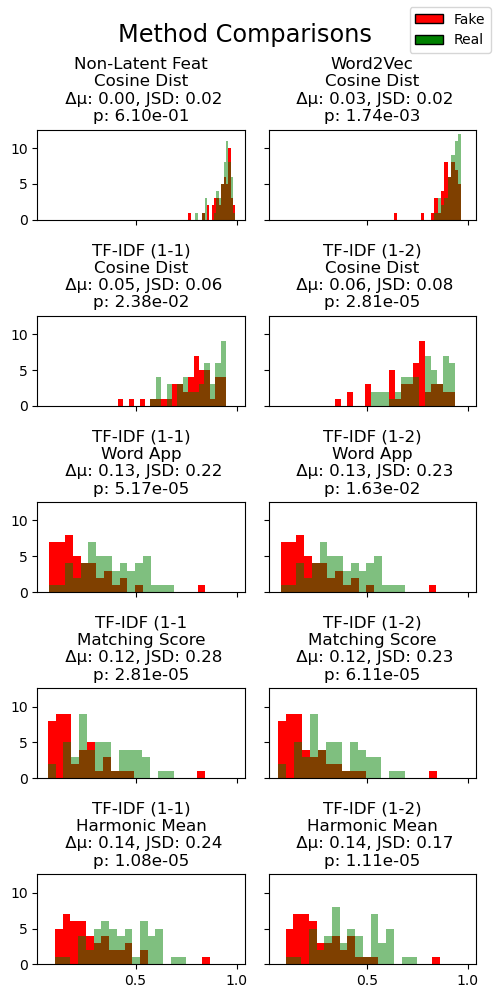
\includegraphics[width=0.5\textwidth]{img/textual_relevance_2.png}
  \caption{Textual Relevance}
  \label{similarity-metrics}
\end{wrapfigure}

\textbf{$\delta \mu$}, or the difference between the mean of \texttt{REAL} and \texttt{FAKE} articles is a very naive and simplistic measure to compare how differentiated the two distributions are. This measure does not remedy the behaviour of outliers which might significantly shift the mean of the distributions. It also ignores the variance of the distributions. However, it is still a numerically simple metric which would aid us when the distributions are well-formed.

\textbf{Jensen-Shannon Divergence (JSD)~\cite{scipy}} is based on the Kullback-Leibler Divergence (KL Divergence) to measure the similarity of two probability distributions. It is symmetric, positive, and in the range of [0, 1] with values closer to 0 denoting more similar distributions and closer to 1 more dissimilar distributions. This is a value we hope to maximise. It is given by the formula:
\[\sqrt{\frac{D(p \parallel m) + D(q \parallel m)}{2}}\]
$D$ is the KL Divergence and $m$ is the \emph{``point-wise mean of p and q''} \cite{scipy}.

\textbf{ANOVA (Analysis of Variance)} is a statistical method to determine if there are significant differences between the means of groups \cite{anova}. We will be performing one-way repeated measure ANOVA which test for any significant difference between the means of the dependent variables (our non-latent features) among the groups defined by the independent variable (our label of \texttt{REAL} and \texttt{FAKE}) to reject the null hypothesis that the group means(\texttt{FAKE} and \texttt{REAL}) are equal. We reject this hypothesis when the p-value associated with the f-statistic of the respetive feature is below the significant level $\alpha = 0.05$.

\subsubsection{Comparison Results}
\tododuke{I can shorten this section if necessary}
Figure~\ref{similarity-metrics} shows our results with similarity metrics comparison. A good metric should have the fake (in red) and the real (in green) distributions be somewhat well separated. The brown area indicates the overlapping region. Non-latent Cosine Distance is the worst metric with $0 \delta \mu$, $0.02 JSD$, and $6.10e-01 p$, where the two \texttt{FAKE} and \texttt{REAL} distributions are overlapping each other almost at the same point. Word2vec Cosine Distance and TF-IDF(1-1) also perform quite poorly with $\delta \mu$ of 0.03 and 0.05, JSD of 0.02 and 0.06, and p-value of 1.74e-03 and 2.38e-02 respectively. Both these plots have the \texttt{REAL} distribution shifted further to the right but the distributions still overlap significantly, unlike the Non-Latent Cosine Distance, however, these metrics fall below the typical significance level $\alpha$ of 0.05. Although TF-IDF (1-2) Cosine Distance has a similar $\delta \mu$ and JSD of 0.06 and 0.08 respectively, its p-value is markedly low at 2.81e-05. Word App follows a similar pattern where TF-IDF (1-1) and (1-2) produce distinctly different results of 5.17e-05 and 1.63e-02 in p-value, but similar $\delta \mu$ of 0.13 and JSD of 0.22 and 0.23 respectively. We can conclude that the ngram-range of TF-IDF definitely contribute to marked differences in the metrics output. Matching score metrics have similar $\delta \mu$ of 0.12 and JSD range of [0.23, 0.28] with low p-values of 2.81e-05 and 6.11e-05 respectively. The most significant features however are the harmonic mean, combining the previous metrics, with TF-IDF (1-1) at $\delta \mu = 0.14, JSD = 0.24, p = 1.08e-05$ and TF-IDF (1-2) at $\delta \mu = 0.14, JSD = 0.17, p = 1.11e-05$. Since TF-IDF (1-1) yields more difference between the distributions, we will use this as our definitive similarity metric.

% \begin{figure}[H]
%   \centering
%     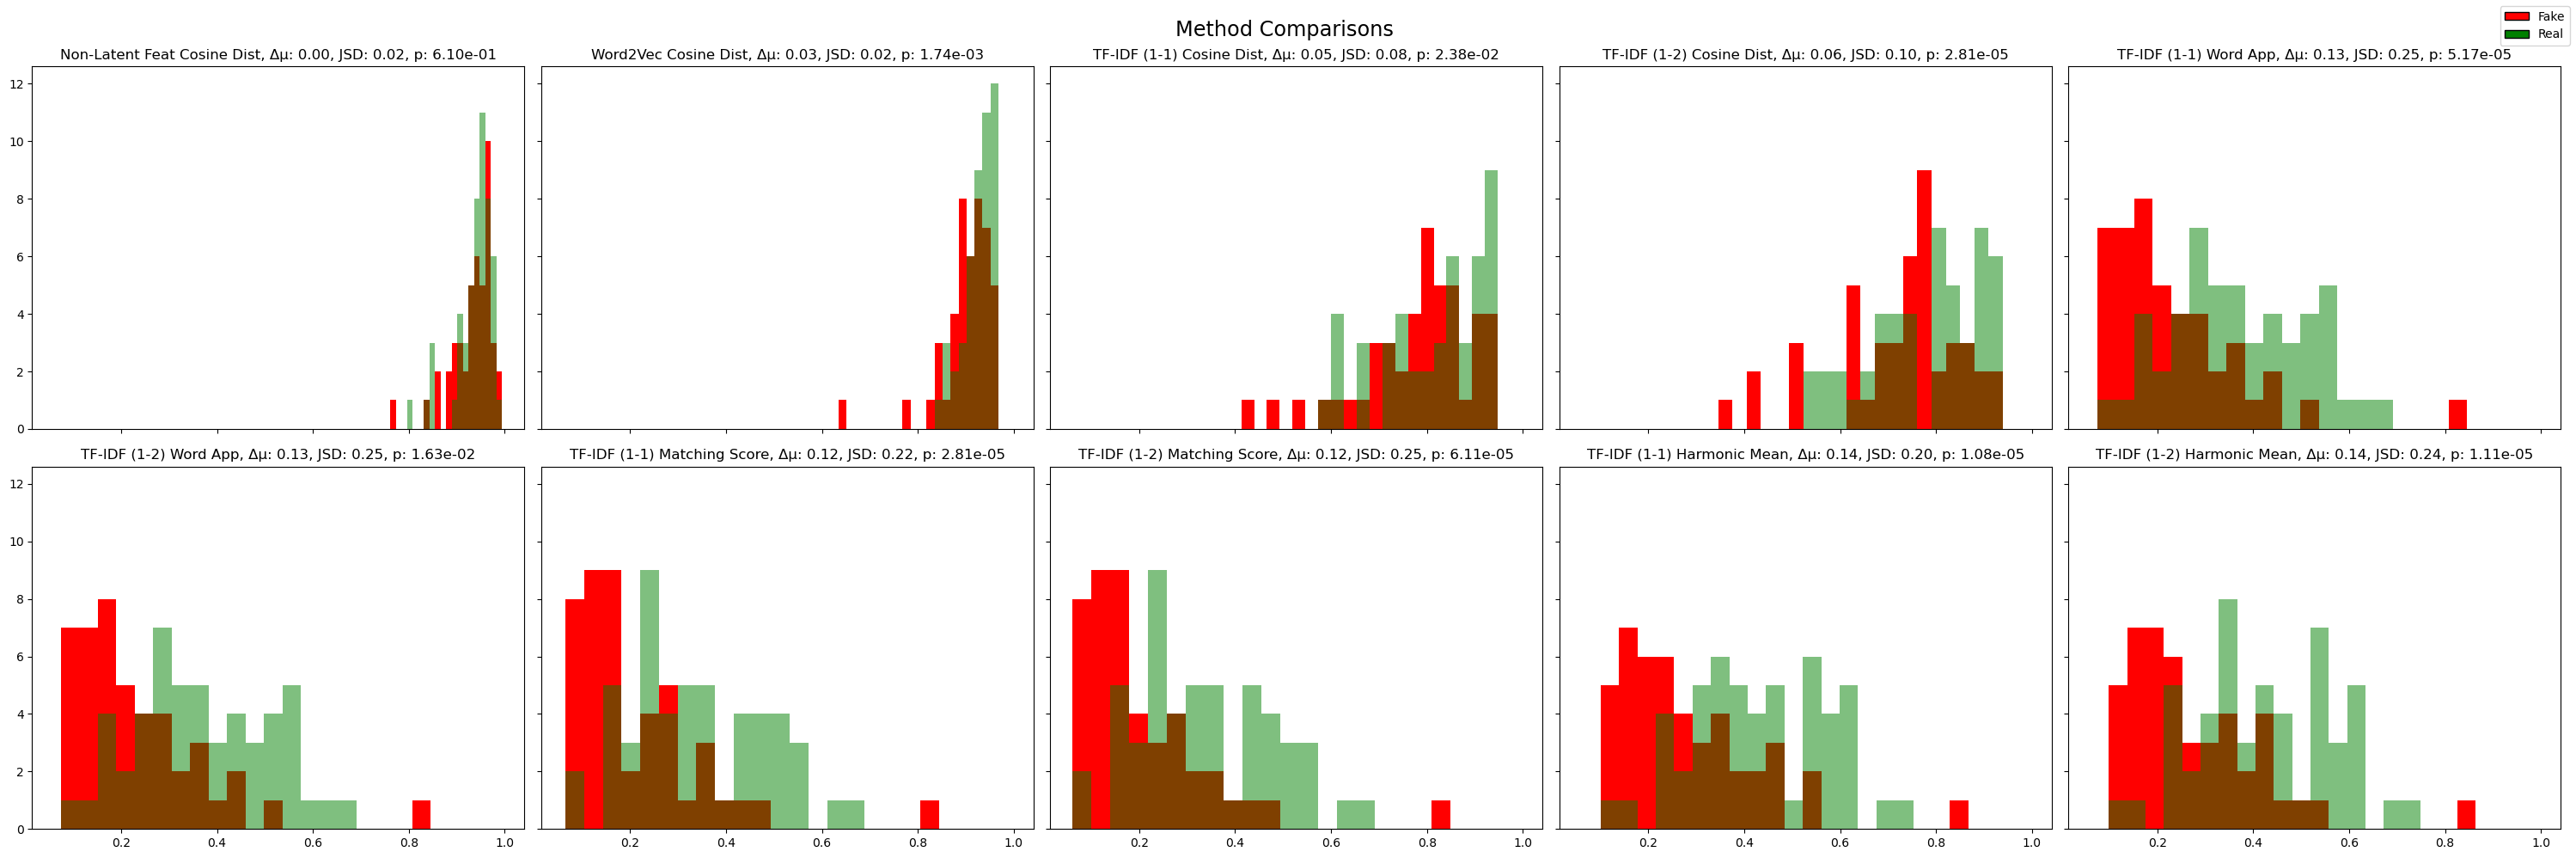
\includegraphics[width=\textwidth]{img/textual_relevance.png}
%     \caption{Textual Relevance}
% \end{figure}

\newsubsection{Feature Normalisation}

\tododhruv{Write}

We experimented with different feature normalisation techniques across the entire dataset and for specific features. Normalisation was conducted columnwise for each feature so that each feature was normalised individually.

\begin{quote}
  \textbf{MinMaxScaler:}\quad This was used for features where there was a clear range of values in order to convert these values into the range of 0-1. This was not implemented frequently across our features as they did not have a fixed range of values making this technique ineffective.

  \textbf{StandardScaler:}\quad This was primarily used for linguistic features that did not have a clear range. This technique works by finding the Z-score for each value within the feature where $\text{Z-score} = \frac{X - \mu}{\sigma}$. This is done by first calculating the mean and standard deviation of the feature and then transforming each value into its Z-score.

  \textbf{RobustScaler:}\quad We experimented with this in place of StandardScaler for values prone to outliers. This was done as RobustScaler uses $\text{IQR} = \text{Q3} - \text{Q1}$ instead of the standard deviation in the transformation calculation from StandardScaler. This is used because standard deviation is highly affected by outlier values and this was noticeable in features such as word count context articles.
\end{quote}

Ultimately, after each scaling technique was applied and the classification was conducted, the results with each type of normalisation and various combinations of them underperformed compared to the original dataset without normalisation. There are a few different reasons why this was the case but after testing various classification models, the most probable reasons are the small size of the dataset used and the lack of appropriate scaling methods available for the linguistic features that rely on counting. Due to this, we decided not to use normalisation for our results.


\newsubsection{Model --- Machine learning}\label{section:machine-learning}

We used four state of the art machine learning models (commonly used in fake news detection) to perform our classification. We chose Logistic Regression (LR), Support Vector Machines (SVM), Decision Trees (DT), and XGBoost (XGB). Due to the small size of our dataset, we needed to tune the regularization hyperparameters to ensure our models didn't overfit. In particular, tree-based models such as DT and XGB should be able to fully segment our classes so we need to control the depth of the tree and splitting criteria. Models such as LR and SVM will need to control L2 regularization. In SVM, we will test the type of kernel used.

To find the best hyperparameters, we perform 5-Fold cross validation across 80\% of our dataset and average the validation score. We pick the parameters with the best validation score and test our model with the remaining 20\% of the dataset. The table in the Appendix~\ref{apppendix:machine-learning} shows the hyperparameters tested for each model and a reason for why the ranges were selected.

\newsubsection{Model --- Neural networks}

\tododhruv{Write}

The second approach taken for classification was using deep learning as we hypothesised that it would be able to find more complex relationships between the large variety of BERT, linguistic, and similarity features. Initially both convolutional neural networks and simple feedforward layers were considered. After analysing the features and noting that they did not have any spacial relation, only the second approach was considered.

We used a very simple structure with 4 hidden layers using the ReLU activation function and an output layer with one neuron and the sigmoid activation function as the task required binary classification. We kept the structure simple due to the small size of the dataset and to prevent overfitting. Additionally, a dropout of 0.2 was added to further prevent overfitting. The dataset was split in a 60:20:20 train, validation, test split to allow for hyperparameter training and binary-crossentropy loss was used. Multiple optimisers were used during training, however, based on the validation accuracy we decided to use Adam as the optimiser.

\newsection{Experimental setup}

\newsubsection{Dataset}\label{section:dataset}

For our research, we use the \verb|FakeNewsData| dataset collated by Horne and Adali in~\cite{horne2017} on research regarding fake news in the 2016 presidential elections. This dataset contains two subsets, \emph{``Buzzfeed Political News''}, and \emph{``Random Political News''}. We make use of the \emph{Buzzfeed} subset since this contains long form text articles that are binary categorized in with Fake and Real labels. The \emph{Random} subset contains an extra label, Satire, which is out of scope for our research.

The original dataset was collated by Craig Silverman (BuzzFeed News Editor) in an article~\cite{dataset-buzzfeed} analyzing fake news. The analysis concentrates on the Facebook engagement on real and fake news articles shared to the social media website. Various keywords related to events during the election were searched and articles with highest engagement were collected. A ground truth was assigned by manual analysis using a list of known fake and hyperpartisan news sites. A details description of their process can be found in their article.

Following BuzzFeed's analysis, Horne extracted the content and title from the articles and formed the dataset. In total, there were 53 real and 48 fake articles. Notable events during the election such as Donald Trump's campaign and various Hillary Clinton scandals and rumors were features in the articles.

After extending this dataset with our novel context article scraping and similarity methods, we used a 60/20/20 train/validation/test set. This was stratified and randomized to ensure the best results. An example of items in our dataset can be found in Table~\ref{article-samples}.

\begin{table}
  \begin{center}
    \makebox[0pt]{\begin{minipage}{\paperwidth}
        \centering
        \subfloat{
          \begin{tabular}{p{8cm}p{8cm}}
            \toprule
            \textbf{118\_Real} & \textbf{1\_Fake}\\
            \midrule
            \emph{\articletitle{118real}} & \emph{\articletitle{1fake}}\\
            \midrule
            \small{\articlecontent{118real}} & \small{\articlecontent{1fake}}\\
            \bottomrule
          \end{tabular}
        }
        \hfill
      \end{minipage}}
  \end{center}
  \caption{A sample of one fake and real article in our dataset. The article ID, title and content are shown in the rows. Both articles are regarding a scandal with Hillary Clinton using a private server to store emails. The fake article reports on an event that never happens whereas the real article reports the true event -- that Clinton was exonerated from criminality.}
  \label{article-samples}
\end{table}

\newsubsection{Data Analysis Using PCA and KMeans}

In order to observe relationships between data within the entire dataset, the BERT, linguistic and similarity features for each data point were collected and dimensionality reduction was conducted using Principle Component Analysis to reduce the dimensions of the data to 2. Plot of these values were constructed with two different combinations of features: one using only BERT features for PCA and the other using linguistic and similarity features in addition to BERT features.

Additionally, to observe whether the data was forming clusters based on its reduced dimensions, KMeans was used with 5 clusters. The reason for using 5 clusters instead of 2 was because both fake and real articles about different topics or written differently can form clusters with other articles in a similar style and we were observing for distinct sets of real and fake clusters rather than simply one region of fake articles and another with real ones.

\begin{figure*}[t!]
  \centering
  \begin{subfigure}[t]{0.5\textwidth}
    \centering
    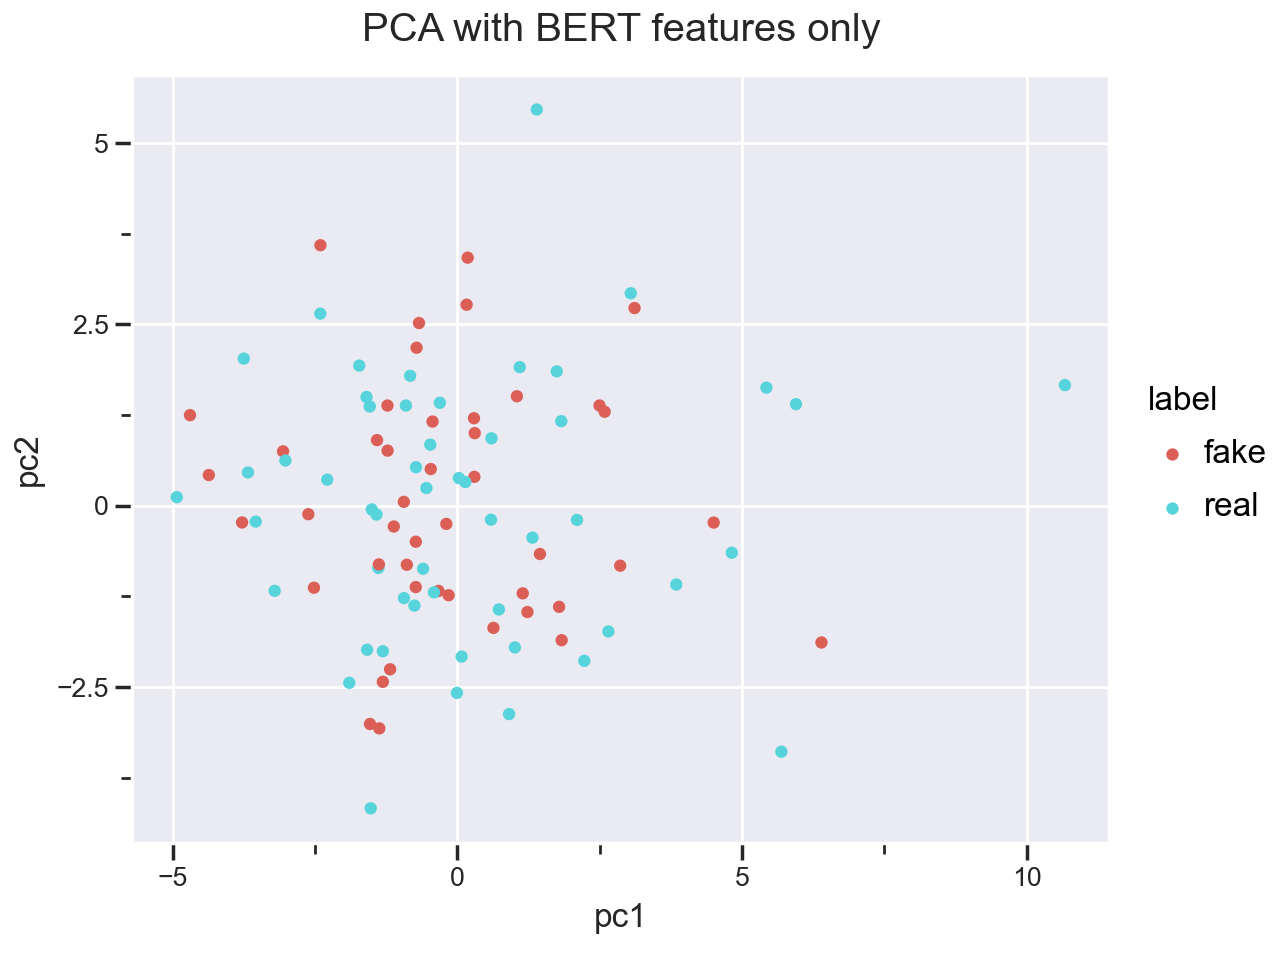
\includegraphics[scale=0.5]{img/pca_1.png}
    \caption{PCA Graph}
    \label{pca_1}
  \end{subfigure}%
  ~
  \begin{subfigure}[t]{0.5\textwidth}
    \centering
    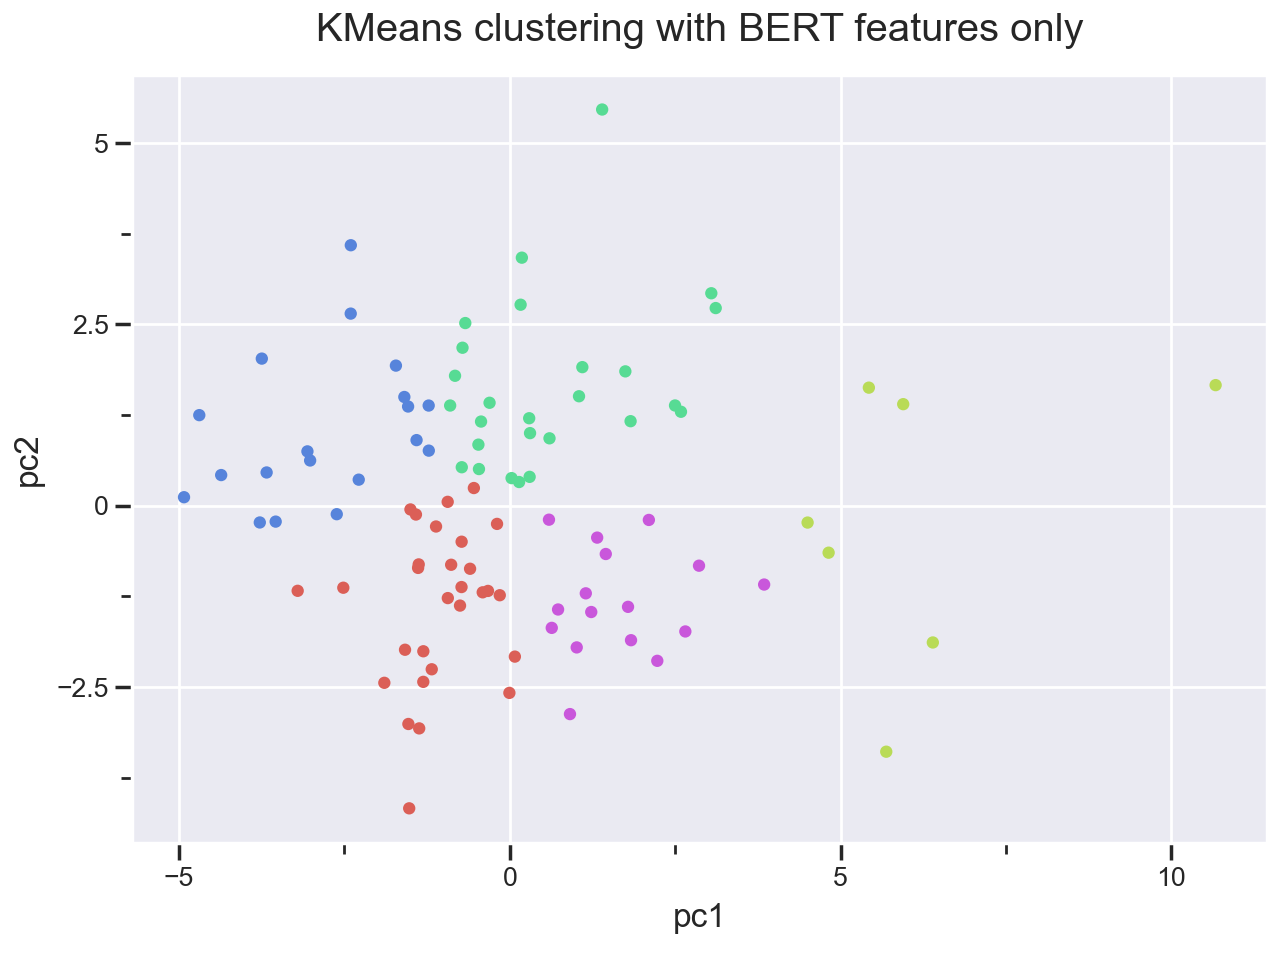
\includegraphics[scale=0.5]{img/kmeans_1.png}
    \caption{KMeans Graph}
    \label{kmeans_1}
  \end{subfigure}
  \caption{Analysis on PCA based on BERT features}
  \label{pca_kmeans_1}
\end{figure*}

\begin{figure*}[t!]
  \centering
  \begin{subfigure}[t]{0.5\textwidth}
    \centering
    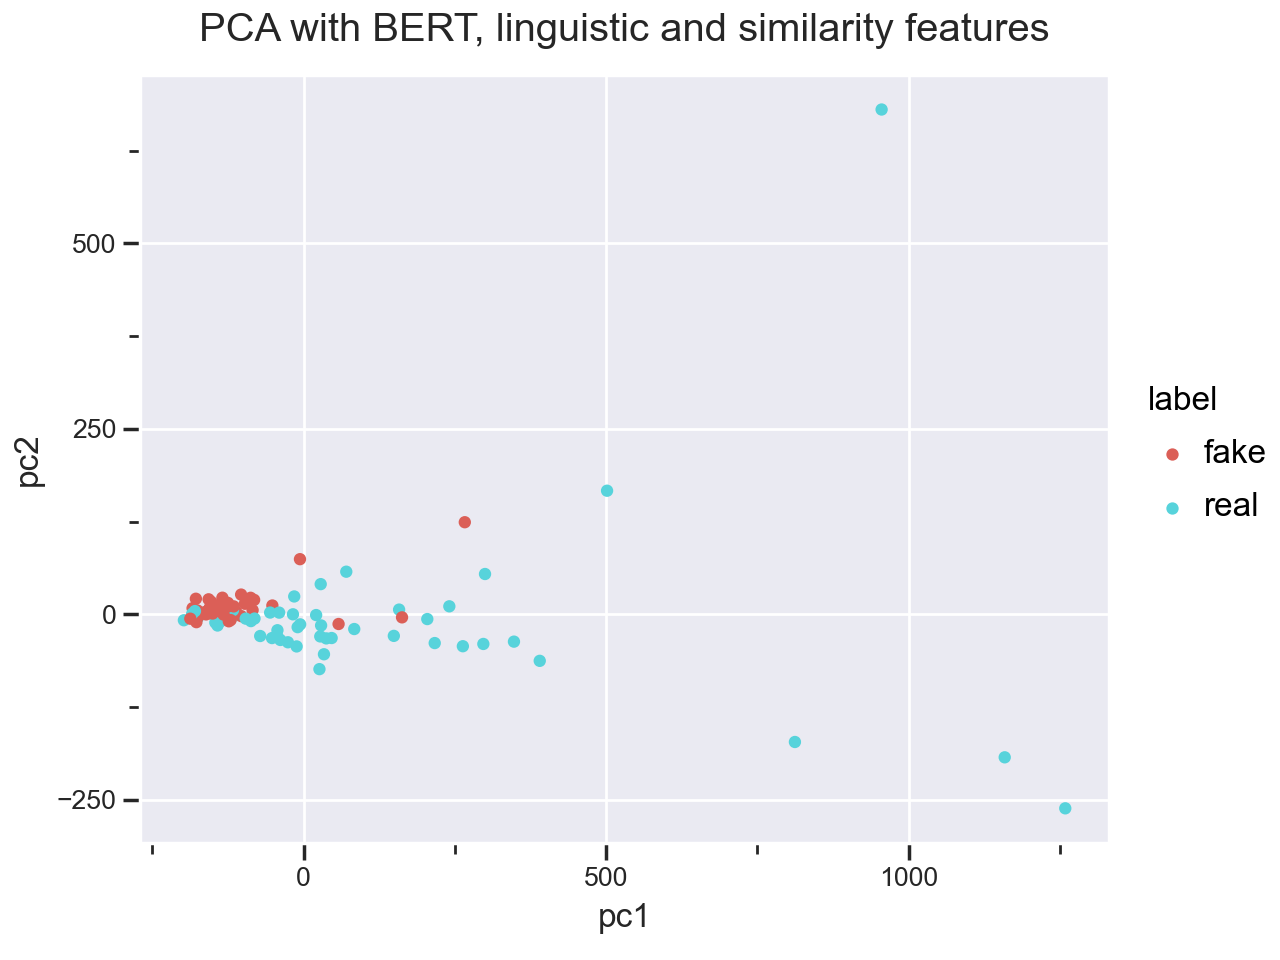
\includegraphics[scale=0.5]{img/pca_3.png}
    \caption{PCA Graph}
    \label{pca_2}
  \end{subfigure}%
  ~
  \begin{subfigure}[t]{0.5\textwidth}
    \centering
    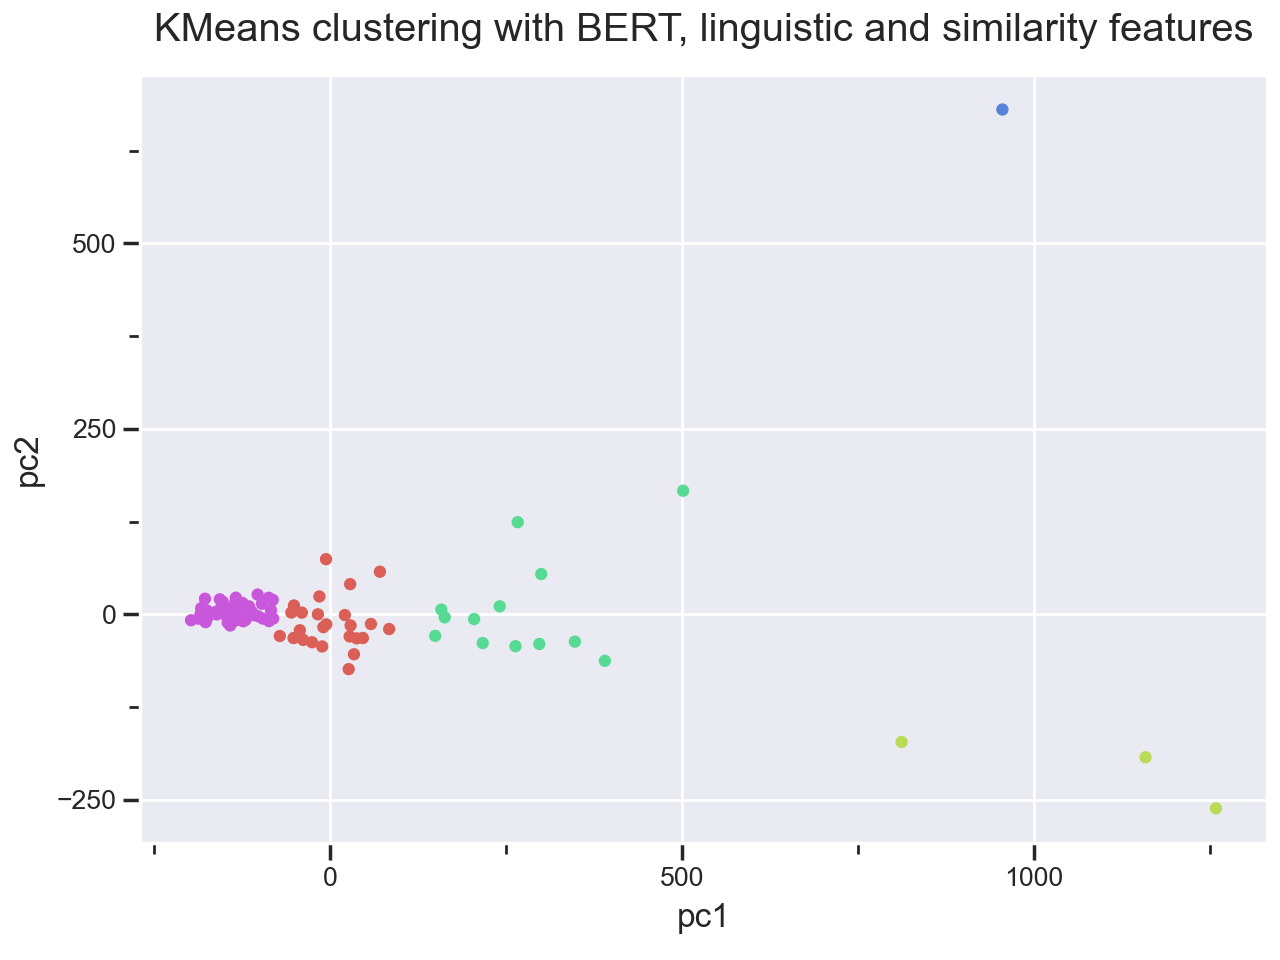
\includegraphics[scale=0.5]{img/kmeans_3.png}
    \caption{KMeans Graph}
    \label{kmeans_2}
  \end{subfigure}
  \caption{Analysis on PCA based on BERT, linguistic and similarity features}
  \label{pca_kmeans_2}
\end{figure*}

As can be seen in Figure \ref{pca_1}, there is very little relationship between the principle components of fake and real articles. When clustering is performed, as shown in Figure \ref{kmeans_1}, each cluster has an even distribution of real and fake articles implying there is no evident pattern in the data.

Whereas in Figure \ref{pca_2}, there is a clear grouping of values for fake data. Interestingly, real data does not have a clear cluster of values and instead occupies a large region of area to the right of the fake data. One potential reason for this is that there are a lot of similar features between fake articles such as the number of adverbs and the types of polarising language. Additionally, the similarity metric could be playing a strong role in influencing the first principle component, pc1, which would potentially result in fake news having low scores and real news having a broader range of similarity scores. Regardless, there is a clear distinction and this is also shown in Figure \ref{kmeans_2} where the majority of fake values are clustered in the purple cluster and the majority of real values are present in two separate clusters.

This indicates that the features selected are effective in separating the dataset into distinct fake and real clusters.

\newsubsection{Evaluation metrics}\label{section:eval}

To evaluate our classification models, we will use accuracy and F1 score. These metrics are commonly used for binary classification problems as well as in the misinformation detection domain. When referring to these metrics, we will label real articles as positive and fake articles as negative.

Accuracy is measured as the proportion of the total number of correctly classified samples over the total count of samples. Mathematically this is represented as
$$\text{Accuracy} = \frac{TP + TN}{TP + TN + FP + FN}.$$

Accuracy is an effective metric for this analysis as it is a holistic measure of the model's ability to identify a real article as real and a fake article as fake, which is the core component of the problem of fake news detection.
Our dataset is quite balanced so this will be a good general first step measure.

Recall refers to how likely the model is able to identify an article is real when its ground truth is real. Precision is a measure of the proportion of all articles the model predicts to be real that have a ground truth of real. As such, recall is a measure of the quantity of the predictions whereas precision is a measure of the quality of the predictions. We are focusing on F1-score as it is the harmonic mean of recall and precision where
$$F_1 = 2\,\frac{\text{precision}\times\text{recall}}{\text{precision}+\text{recall}}.$$

This allows for a fair assessment of both the quantity and quality of the predictions in a format that makes it easier to compare both models.

\newsection{Results and discussion}

\tododhruv{Add intro to results}
\begin{comment}
For our machine learning models, we observed a increase in accuracy and F1 as we added our higher quality features to the model. Table~\ref{machine-learning-results} shows our results for all models.

With just the BERT features, all our chosen models performed not much better than random guessing with XGBoost edging out with a 0.6 F1 score. This shows that just the bert features themselves don't convey enough information by themselves when fitting weights to our models.

When we add our selected non-latent features, we see a large jump in performance in all models. In particular, we see XGB remain strong due to its ability to select the best features to split on and SVC becoming our best performer.

Adding our novel similarity score, we see more improvement. XGB and DT have improved by a large amount with XGB as our best performer. This is due to the fact that our similarity is one feature amount about 800 features and we know both these models are able to select the best feature for splitting. We also see that SVC and LR have stagnated after adding this score but have not decreased in performance due to not being able to make effective use of this single feature.

\end{comment}


For our analysis, we will be comparing the top 3 performing machine learning methods alongside the best performing neural network for each task. There are three models that are compared

\begin{enumerate}
  \item \textbf{Model 1} is trained only on BERT features
  \item \textbf{Model 2} is trained on both BERT and linguistic features
  \item \textbf{Model 3} is trained on BERT, linguistic and similarity features
\end{enumerate}

\begin{figure}[!hbp]
  \centering
  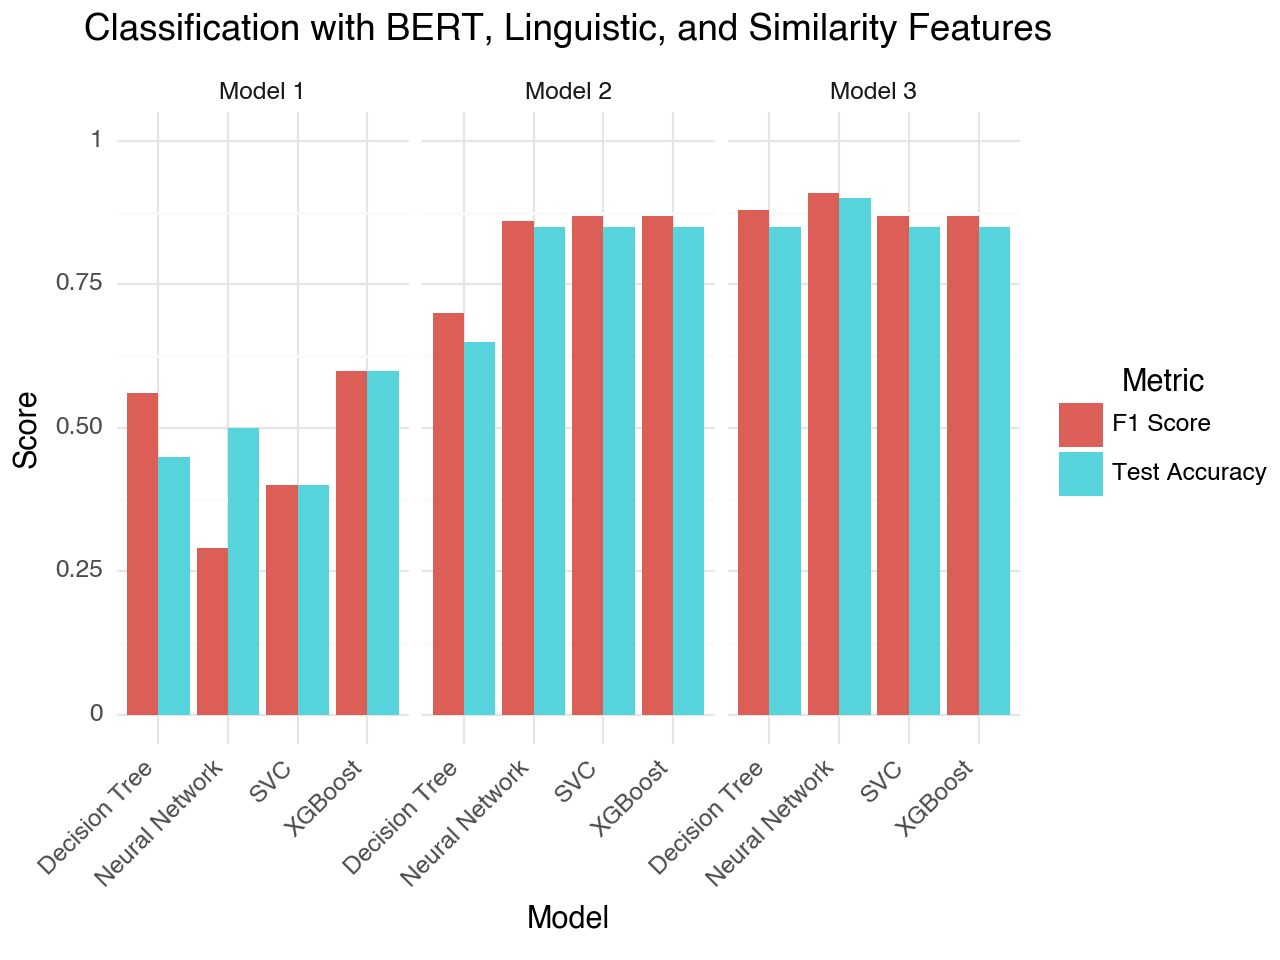
\includegraphics[]{img/accuracy_combined_graph.png}
  \caption{Accuracy and F1-score metrics for top performing models across different features}
  \label{accuracy_graph}
\end{figure}

Figure \ref{accuracy_graph} presents the classification results. As hypothesised from dataset analysis with PCA, Model 1 does not perform well. With a testing accuracy around 50\% for each classifier, it is simply random guessing on the data. This is used as the baseline for our analysis as it is does incorporate any of our novel contribution to this knowledge domain.

Model 2 incorporates the most effective linguistic features in addition to the BERT features from Model 1. There is a significant increase in testing accuracy and F1-score across every model. Evident in the more complex models of neural networks and XGBoost, it is clear that there is a complex relationship being captured. The increase in accuracy to around

\begin{comment}
\begin{figure}[!hbp]
  \centering
  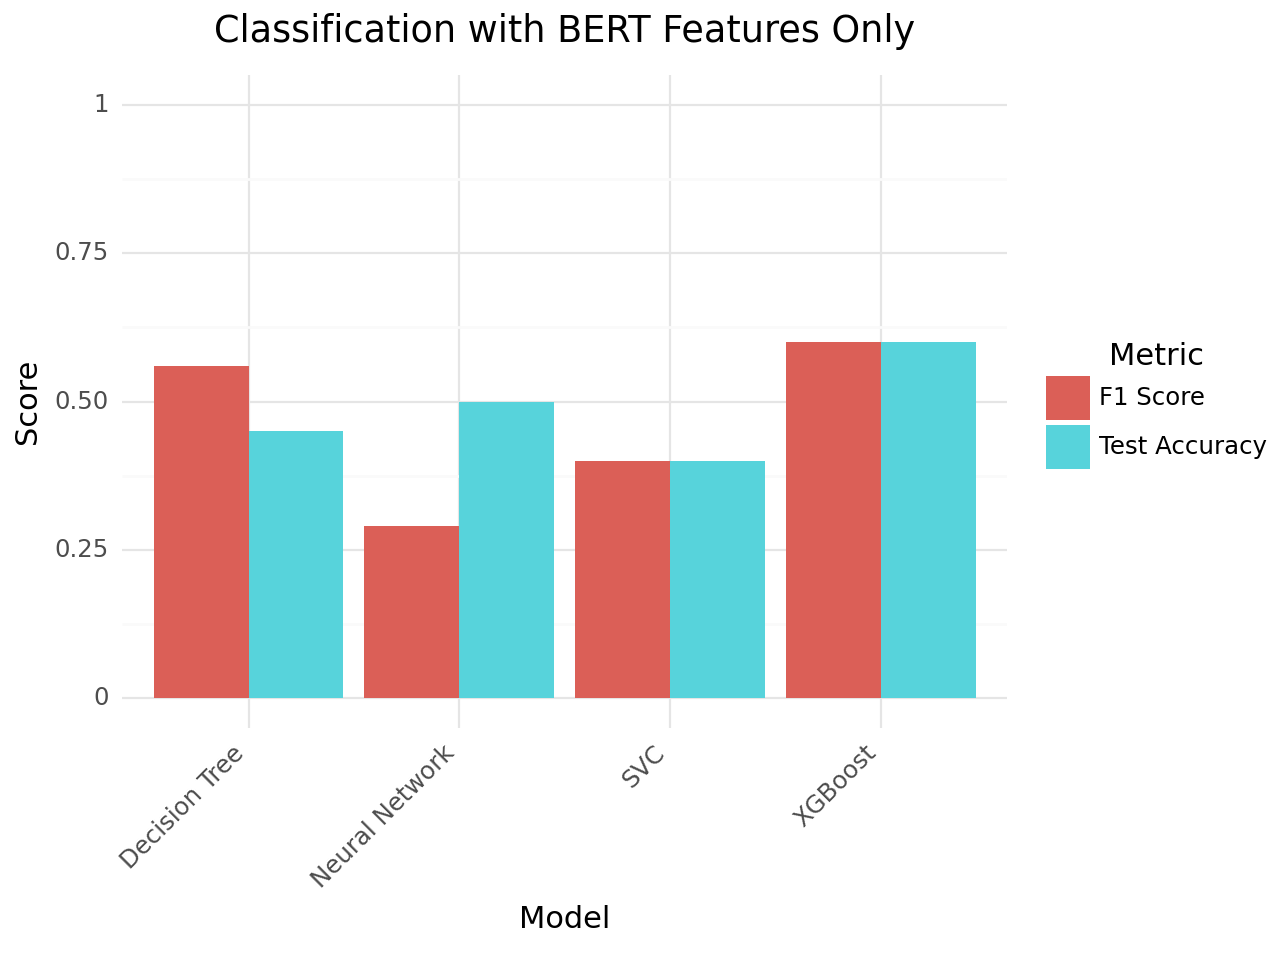
\includegraphics[]{img/accuracy_graph_1.png}
  \caption{Metrics for models based on BERT features}
  \label{accuracy_graph_1}
\end{figure}

As we can see from Figure \ref{accuracy_graph_1}, each model performs very poorly when the input is simply the BERT features and no linguistic or similarity metrics are used.

\begin{figure}[!hbp]
  \centering
  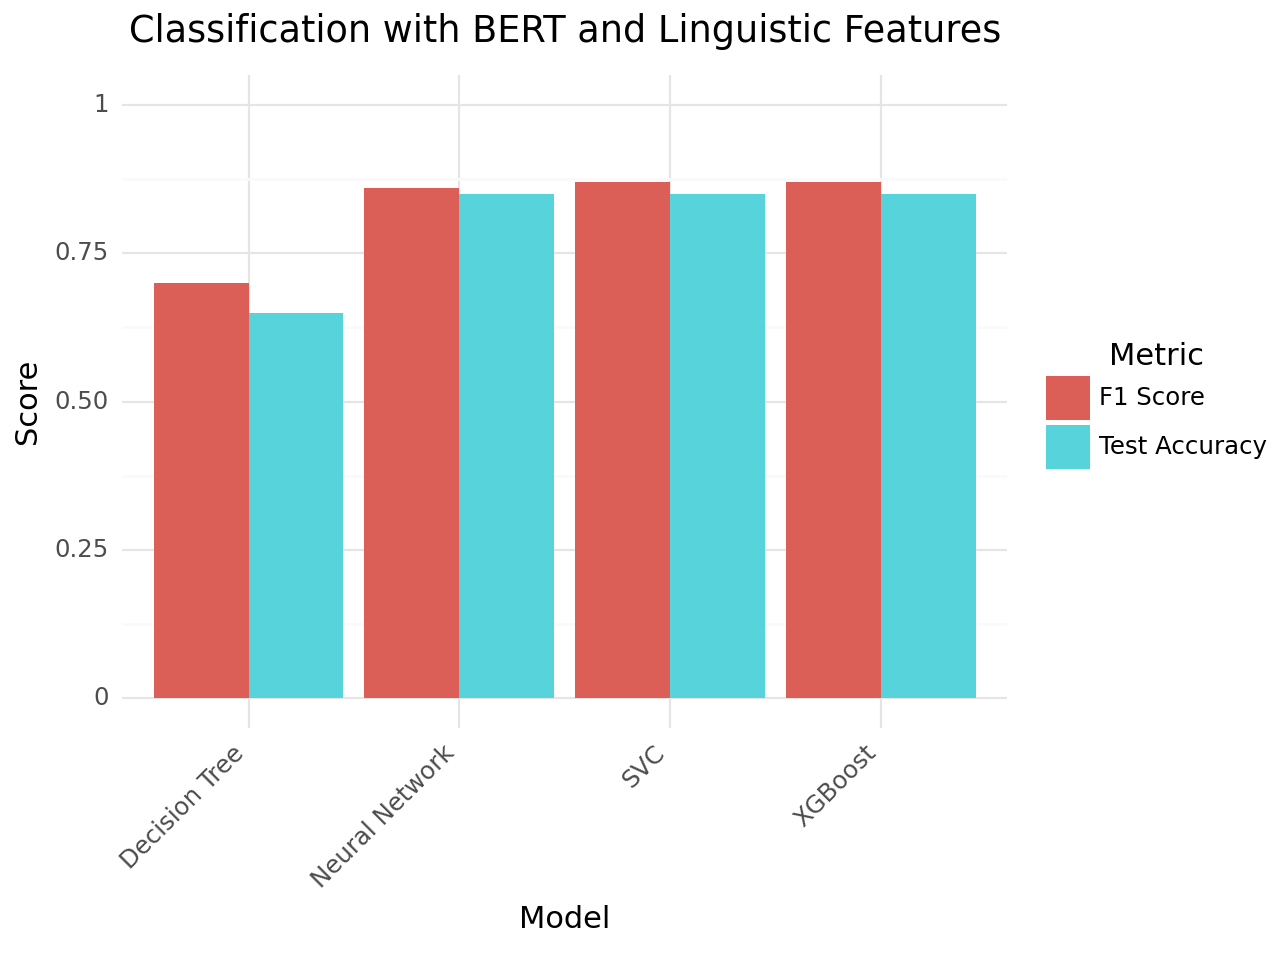
\includegraphics[]{img/accuracy_graph_2.png}
  \caption{Metrics for models based on BERT and linguistic features}
  \label{accuracy_graph_2}
\end{figure}

After incorporating linguistic features, shown in Figure \ref{accuracy_graph_2} there is a noticeable improvement across all

\begin{figure}[!hbp]
  \centering
  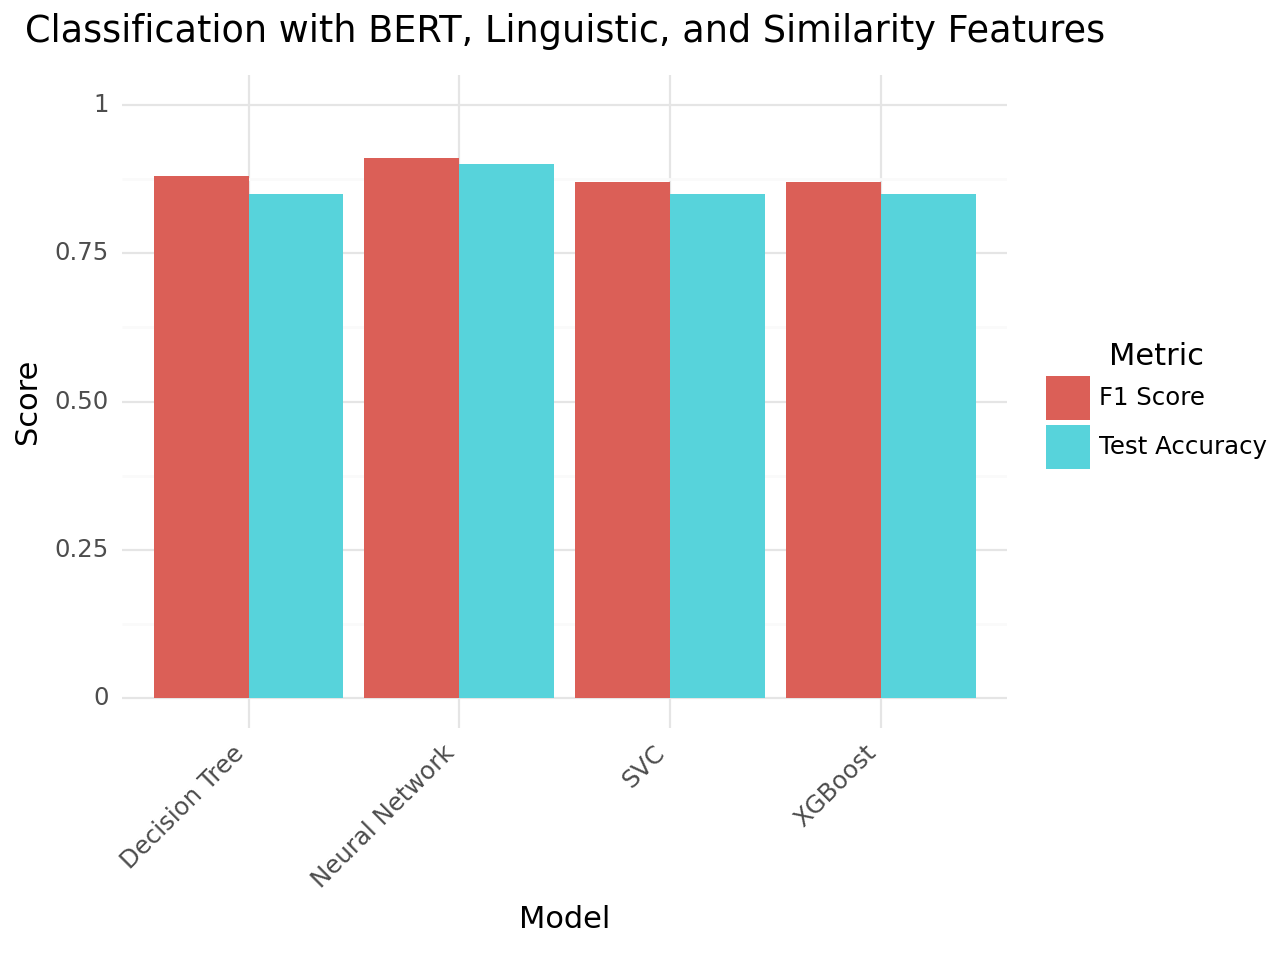
\includegraphics[]{img/accuracy_graph_3.png}
  \caption{Metrics for models based on BERT features}
\end{figure}
\end{comment}

\begin{table}
  \centering
  \begin{tabular}{cccccc}
    \toprule
    Features & Model & Train Acc. & Train F1 & Test Acc. & Test F1\\
    \midrule
    \multirow{4}{*}{BERT} & LR & 0.99 & 0.99 & 0.5 & 0.5\\
    \cmidrule{2-6}
    & SVC & 1.0 & 1.0 & 0.4 & 0.4\\
    \cmidrule{2-6}
    & DT & 0.99 & 0.99 & 0.45 & 0.56\\
    \cmidrule{2-6}
    & \textbf{XGB} & 1.0 & 1.0 & \textbf{0.6} & \textbf{0.6}\\
    \midrule
    \multirow{4}{*}{\shortstack{BERT\\+ Non-Latent}} & LR & 0.94 & 0.94 & 0.70 & 0.73\\
    \cmidrule{2-6}
    & \textbf{SVC} & 0.79 & 0.79 & \textbf{0.85} & \textbf{0.87}\\
    \cmidrule{2-6}
    & DT & 1.0 & 1.0 & 0.65 & 0.70\\
    \cmidrule{2-6}
    & \textbf{XGB} & 1.0 & 1.0 & \textbf{0.85} & \textbf{0.87}\\
    \midrule
    \multirow{4}{*}{\shortstack{BERT\\+ Non-Latent\\+ Similarity}} & LR & 0.94 & 0.94 & 0.7 & 0.73\\
    \cmidrule{2-6}
    & SVC & 0.79 & 0.79 & 0.85 & 0.87\\
    \cmidrule{2-6}
    & \textbf{DT} & 1.0 & 1.0 & \textbf{0.85} & \textbf{0.88}\\
    \cmidrule{2-6}
    & XGB & 1.0 & 1.0 & 0.85 & 0.87\\
    \bottomrule
  \end{tabular}
  \caption{Table showing all training and test accuracies and F1 scores on our machine learning models with different feature inputs. The best test accuracy and F1 score have been emboldened.}
  \label{machine-learning-results}
\end{table}

\todojim{Add table of parameters of models}

\tododhruv{Neural nets}

\newsection{Conclusion}

\todoany{Summarise the study and discuss directions for future improvement}

\newsubsection{Limitations}

\todoany{Convert list of limitations to subsubsections with discussion.}

\subsubsection*{Preprocessing and tokenization}\label{limitation:preprocessing}

While our preprocessing was quite generic for NLP tasks, we believe there were a few oversights that caused unreliable results. Two issues were:
\begin{itemize}
  \item Converting everything to lowercase destroyed acronyms such as ``US''. This changed the meaning of some sentences.
  \item The \verb|nltk| lemmatizer required manually specifying the part of speech to work. This caused some verbs to be incorrectly lemmatized. We could have used a different library that extracted the POS automatically. Alternatively we could have investigated not lemmatizing at all to maintain proper structure for non-latent features and BERT embeddings.
\end{itemize}

This research would have really benefitted from less or no preprocessing at all. For all our features, there could be an argument where no preprocessing would have been better. For example summary extraction or BERT features could have learnt meaning from the unfiltered text. This could be investigated for future research to strengthen our features.

\subsubsection*{Summary extraction}\label{limitation:summary-extraction}

Our summary extraction extracted most of the correct meaning from the text. However two main issues remained causing it to produce in-perfect results:
\begin{itemize}
  \item Words would be unordered and if read together in a sentence, wouldn't make sense to a human.
  \item \emph{Junk} such as connectives would be left in the summary.
\end{itemize}

We believe future research could have looked into better tuned models that synthesized higher quality topic sentences. In our research, there were very few but we believe in particular a summary extractor trained on long-form news articles would have performed better. In addition, we could have also included the title since semantically, the title is supposed to tell the reader what the rest of the article is about.

\subsubsection*{Article scraping}\label{limitation:article-scraping}

We had intended our pipeline to be fully automatic, using an API to scrape for articles based on the keywords. For the scope of this project, we settled on manual scraping to show that using contextual articles would improve results. Unfortunately, after being passed to Google, some input summaries would return no or limited results and required human intervention to produce any articles. This was a particular problem.

For Real labelled articles, we believe an improvement on the summary extractor reducing the amount of \emph{junk} returned would have improved results. However, we hypothesize that if an outrageous Fake article as introduced, we may very well find no results about the event online. One example is the following article about Trump \emph{``snorting cocaine''}:
\begin{quote}
  \textbf{10Fake:}\quad\articlecontent{10fake}
\end{quote}
This event never happened and consequently, we could not find any contextual articles about it. For our research, we skipped articles with no context. We believe one way to resolve this is to include the article with no similarity score or a low one. More research needs to be done into whether mixed articles with and without a similarity can perform well together especially considering in the real world, this is definatly an issue.

\subsubsection*{Dataset}

For the scope of our research, we used a fairly small dataset to present our contributions to contextual article scraping. However, this dataset only concentrated on the political events surrounding the 2016 United States election. This causes two main problems for our model:
\begin{itemize}
  \item We are prone to overfit our models since such a small dataset will be easily segmented by most state of the art methods.
  \item Our model will learn specifics in the US election which we do not want to learn. This could cause the models to be confused if we try to classify more recent news.
\end{itemize}

In the future research could be done to provide an automated API for scraping which would have allowed for a much larger dataset to be used that covers multiple world events across different years. Along with this, masking out event specific words could have been done to reduce learning of event specifics.

\newsubsection{Future work}
\tododuke{Talk about doing average pooling of the entire output for future work instead of just using the CLS token}
\tododuke{Future work: vectorise the title and not just the body (non-latent + similarity)}
\tododuke{Future work: detect similarity between body and title pair (similarity)}
\tododuke{Future work: learn a model instead of using metrics (similarity)}

\cleardoublepage
\pagebreak

\nocite{*}
\printbibliography

\cleardoublepage
\pagebreak

\appendix

\newsection{Individual contributions}

\begin{table}[H]
  \centering
  \begin{tabular}{cp{{7cm}}}
    \toprule
    Member & Major contributions to project and report\\
    \midrule
    Jim & \shortstack{Proprocessing \& tokenization\\Similarity model article scraping\\Machine learning models}\\
    \midrule
    Dhruv & \\
    \midrule
    Duke & \\
    \bottomrule
  \end{tabular}
\end{table}

\subsection{Jim}

Jim contributed to the project particularly in the sections of preprocessing \& tokenization, similarity model (Article Scraping), and the machine learning models. At the start of the project Jim contributed to the manual scraping of articles. Towards the end of the project, Jim was also responsible for writing code to combine all the features together and integrating all work completed by the other members so that models can be run using common bootstrap code.

In the project proposal and literature review, Jim contributed equally with the team and worked on each other's sections. In the project demo, Jim contributed less than average due to the fact that a live online demo was cut from the final version due to time and validity reasons. It was decided that since the rest of the team already started their assigned sections, Jim would start on the report and attempt to contribute more than average.

In the report Jim contributed to the Sections~\ref{section:preprocessing}, \ref{section:summary-extraction}, \ref{section:article-scraping}, \ref{section:machine-learning}, \ref{section:dataset}, \ref{section:eval}, the machine learning part in results and related limitations.

\subsection{Dhruv}

\tododhruv{$\sim$1pg detailing individual contributions}

\subsection{Duke}

\tododuke{$\sim$1pg detailing individual contributions}

\newsection{Article scraping}\label{appendix:article-scraping}

\begin{table}[H]
  \centering
  \begin{tabular}{cp{8cm}p{3cm}}
    \toprule
    ID & Article extract & Summary\\
    \midrule
    \verb|128_Real| & \small{\articlecontent{128real}} & god wa one never every king november still heart\\
    \midrule
    \verb|2_Fake| & \small{\articlecontent{2fake}} & ha adenugame africanamericans south femi united states africa president donald\\
    \midrule
    \verb|10_Fake| & \small{\articlecontent{10fake}} &wa room hotel maria told employee gonzalez hit video get\\
    \midrule
    \verb|34_Fake| & \small{\articlecontent{34fake}} &trump rage album machine band ha donald music outside year\\
    \bottomrule
  \end{tabular}
  \caption{Articles we were not able to find context articles for.}
\end{table}

\newsection{Non-Latent Features}\label{appendix:non-latent-table}
 \begin{longtable}[c]{| >{\centering\arraybackslash}p{.2\textwidth} | >{\centering\arraybackslash}p{.3\textwidth} | >{\centering\arraybackslash}p{.13\textwidth} | >{\centering\arraybackslash}p{.25\textwidth} |}
\hline
\textbf{Category}                  & \textbf{Feature Type}                & \textbf{Calculation}      & \textbf{Feature Name}       \\ \hline
\multirow{14}{*}{Diversity}        & Noun (Unique)                        & \multirow{7}{*}{Count}    & div\_NOUN\_sum              \\ \cline{2-2} \cline{4-4} 
                                   & Verb (Unique)                        &                           & div\_VERB\_sum              \\ \cline{2-2} \cline{4-4} 
                                   & Adjective (Unique)                   &                           & div\_ADJ\_sum               \\ \cline{2-2} \cline{4-4} 
                                   & Adverb (Unique)                      &                           & div\_ADV\_sum               \\ \cline{2-2} \cline{4-4} 
                                   & Lexical Word (Unique)                &                           & div\_LEX\_sum               \\ \cline{2-2} \cline{4-4} 
                                   & Content Word (Unique)                &                           & div\_CONT\_sum              \\ \cline{2-2} \cline{4-4} 
                                   & Function Word (Unique)               &                           & div\_FUNC\_sum              \\ \cline{2-4} 
                                   & Noun (Unique)                        & \multirow{7}{*}{Percent}  & div\_NOUN\_percent          \\ \cline{2-2} \cline{4-4} 
                                   & Verb (Unique)                        &                           & div\_VERB\_percent          \\ \cline{2-2} \cline{4-4} 
                                   & Adjective (Unique)                   &                           & div\_ADJ\_percent           \\ \cline{2-2} \cline{4-4} 
                                   & Adverb (Unique)                      &                           & div\_ADV\_percent           \\ \cline{2-2} \cline{4-4} 
                                   & Lexical Word (Unique)                &                           & div\_LEX\_percent           \\ \cline{2-2} \cline{4-4} 
                                   & Content Word (Unique)                &                           & div\_CONT\_percent          \\ \cline{2-2} \cline{4-4} 
                                   & Function Word (Unique)               &                           & div\_FUNC\_percent          \\ \hline
\multirow{42}{*}{Quantity}         & Noun                                 & \multirow{18}{*}{Count}   & div\_NOUN\_sum              \\ \cline{2-2} \cline{4-4} 
                                   & Verb                                 &                           & div\_VERB\_sum              \\ \cline{2-2} \cline{4-4} 
                                   & Adjective                            &                           & div\_ADJ\_sum               \\ \cline{2-2} \cline{4-4} 
                                   & Adverb                               &                           & div\_ADV\_sum               \\ \cline{2-2} \cline{4-4} 
                                   & Pronoun                              &                           & div\_PRON\_sum              \\ \cline{2-2} \cline{4-4} 
                                   & Personal Pronoun                     &                           & div\_DET\_sum               \\ \cline{2-2} \cline{4-4} 
                                   & Possessive Pronoun                   &                           & div\_NUM\_sum               \\ \cline{2-2} \cline{4-4} 
                                   & Determinant                          &                           & div\_PUNCT\_sum             \\ \cline{2-2} \cline{4-4} 
                                   & Number                               &                           & div\_SYM\_sum               \\ \cline{2-2} \cline{4-4} 
                                   & Punctuation                          &                           & div\_PRP\_sum               \\ \cline{2-2} \cline{4-4} 
                                   & Symbol                               &                           & div\_PRP\$\_sum             \\ \cline{2-2} \cline{4-4} 
                                   & Wh-Determinant                       &                           & div\_WDT\_sum               \\ \cline{2-2} \cline{4-4} 
                                   & Cardinal Number                      &                           & div\_CD\_sum                \\ \cline{2-2} \cline{4-4} 
                                   & Verb (Past Tense)                    &                           & div\_VBD\_sum               \\ \cline{2-2} \cline{4-4} 
                                   & Stop Word                            &                           & div\_STOP\_sum              \\ \cline{2-2} \cline{4-4} 
                                   & Lowercase Word                       &                           & div\_LOW\_sum               \\ \cline{2-2} \cline{4-4} 
                                   & Uppercase Word                       &                           & div\_UP\_sum                \\ \cline{2-2} \cline{4-4} 
                                   & Negation                             &                           & div\_NEG\_sum               \\ \cline{2-4} 
                                   & Noun                                 & \multirow{18}{*}{Percent} & div\_NOUN\_percent          \\ \cline{2-2} \cline{4-4} 
                                   & Verb                                 &                           & div\_VERB\_percent          \\ \cline{2-2} \cline{4-4} 
                                   & Adjective                            &                           & div\_ADJ\_percent           \\ \cline{2-2} \cline{4-4} 
                                   & Adverb                               &                           & div\_ADV\_percent           \\ \cline{2-2} \cline{4-4} 
                                   & Pronoun                              &                           & div\_PRON\_percent          \\ \cline{2-2} \cline{4-4} 
                                   & Personal Pronoun                     &                           & div\_DET\_percent           \\ \cline{2-2} \cline{4-4} 
                                   & Possessive Pronoun                   &                           & div\_NUM\_percent           \\ \cline{2-2} \cline{4-4} 
                                   & Determinant                          &                           & div\_PUNCT\_percent         \\ \cline{2-2} \cline{4-4} 
                                   & Number                               &                           & div\_SYM\_percent           \\ \cline{2-2} \cline{4-4} 
                                   & Punctuation                          &                           & div\_PRP\_percent           \\ \cline{2-2} \cline{4-4} 
                                   & Symbol                               &                           & div\_PRP\$\_percent         \\ \cline{2-2} \cline{4-4} 
                                   & Wh-Determinant                       &                           & div\_WDT\_percent           \\ \cline{2-2} \cline{4-4} 
                                   & Cardinal Number                      &                           & div\_CD\_percent            \\ \cline{2-2} \cline{4-4} 
                                   & Verb (Past Tense)                    &                           & div\_VBD\_percent           \\ \cline{2-2} \cline{4-4} 
                                   & Stop Word                            &                           & div\_STOP\_percent          \\ \cline{2-2} \cline{4-4} 
                                   & Lowercase Word                       &                           & div\_LOW\_percent           \\ \cline{2-2} \cline{4-4} 
                                   & Uppercase Word                       &                           & div\_UP\_percent            \\ \cline{2-2} \cline{4-4} 
                                   & Negation                             &                           & div\_NEG\_percent           \\ \cline{2-4} 
                                   & Quote                                & \multirow{6}{*}{Count}    & div\_QUOTE\_sum             \\ \cline{2-2} \cline{4-4} 
                                   & Noun Phrase                          &                           & div\_NP\_sum                \\ \cline{2-2} \cline{4-4} 
                                   & Character                            &                           & div\_CHAR\_sum              \\ \cline{2-2} \cline{4-4} 
                                   & Word                                 &                           & div\_WORD\_sum              \\ \cline{2-2} \cline{4-4} 
                                   & Sentence                             &                           & div\_SENT\_sum              \\ \cline{2-2} \cline{4-4} 
                                   & Syllable                             &                           & div\_SYLL\_sum              \\ \hline
\multirow{5}{*}{Sentiment}         & Exclamation Mark                     & \multirow{3}{*}{Count}    & div\_!\_sum                 \\ \cline{2-2} \cline{4-4} 
                                   & Question Mark                        &                           & div\_?\_sum                 \\ \cline{2-2} \cline{4-4} 
                                   & All-Cap Word                         &                           & div\_CAPS\_sum              \\ \cline{2-4} 
                                   & Polarity                             & \multirow{2}{*}{Index}    & div\_POL\_sum               \\ \cline{2-2} \cline{4-4} 
                                   & Subjectivity                         &                           & div\_SUBJ\_sum              \\ \hline
\multirow{6}{*}{Pronoun}           & First Person Singular                & \multirow{3}{*}{Count}    & div\_FPS\_sum               \\ \cline{2-2} \cline{4-4} 
                                   & First Person Plural                  &                           & div\_FPP\_sum               \\ \cline{2-2} \cline{4-4} 
                                   & Second / Third Person                &                           & div\_STP\_sum               \\ \cline{2-4} 
                                   & First Person Singular                & \multirow{3}{*}{Percent}  & div\_FPS\_percent           \\ \cline{2-2} \cline{4-4} 
                                   & First Person Plural                  &                           & div\_FPP\_percent           \\ \cline{2-2} \cline{4-4} 
                                   & Second / Third Person                &                           & div\_STP\_percent           \\ \hline
\multirow{4}{*}{Average}           & Character Per Word                   & \multirow{4}{*}{Average}  & div\_chars\_per\_word\_sum  \\ \cline{2-2} \cline{4-4} 
                                   & Word Per Sentence                    &                           & div\_words\_per\_sent\_sum  \\ \cline{2-2} \cline{4-4} 
                                   & Clause Per Sentence                  &                           & div\_claus\_per\_sent\_sum  \\ \cline{2-2} \cline{4-4} 
                                   & Punctuation Per Sentence             &                           & div\_puncts\_per\_sent\_sum \\ \hline
\multirow{2}{*}{Syntax Tree Depth} & Median Syntax Tree Depth             & \multirow{2}{*}{Median}   & div\_ALL\_sum               \\ \cline{2-2} \cline{4-4} 
                                   & Median Noun Phrase Syntax Tree Depth &                           & div\_NP\_sum                \\ \hline
\multirow{8}{*}{Readability}       & Gunning-Fog Index                    & \multirow{8}{*}{Index}    & div\_gunning-fog\_sum       \\ \cline{2-2} \cline{4-4} 
                                   & Coleman-Liau Index                   &                           & div\_coleman-liau\_sum      \\ \cline{2-2} \cline{4-4} 
                                   & Flesch Kincaid Grade Level           &                           & div\_dale-chall\_sum        \\ \cline{2-2} \cline{4-4} 
                                   & Linsear Write                        &                           & div\_flesch-kincaid\_sum    \\ \cline{2-2} \cline{4-4} 
                                   & SPACHE                               &                           & div\_linsear-write\_sum     \\ \cline{2-2} \cline{4-4} 
                                   & Dale Chall Readability               &                           & div\_spache\_sum            \\ \cline{2-2} \cline{4-4} 
                                   & Automated Readability Index (ARI)    &                           & div\_automatic\_sum         \\ \cline{2-2} \cline{4-4} 
                                   & Flesch Reading Ease                  &                           & div\_flesch\_sum            \\ \hline
\end{longtable}

\newsection{Non-latent Feature Pearson Correlation Matrix}\label{appendix:correlation-matrx}
\begin{figure}[H]
  \centering
  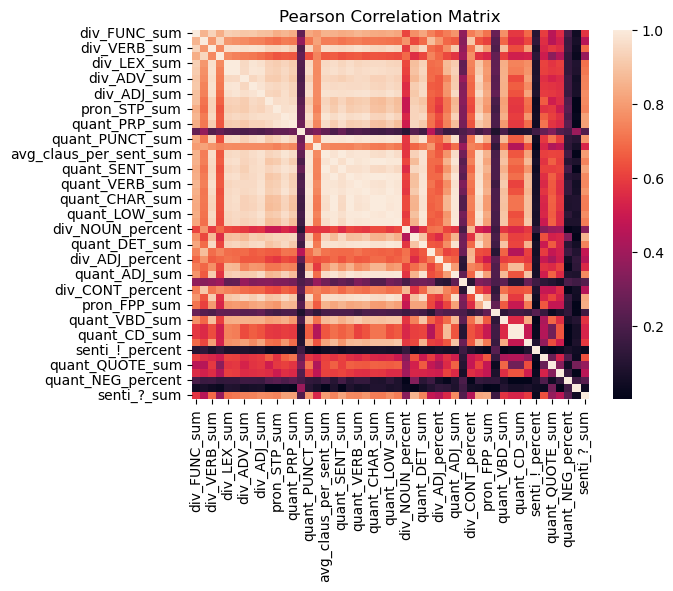
\includegraphics[width=0.8\textwidth]{img/non_latent_corr_matrx.png}
  \caption{Non-Latent Correlation Matrix}
\end{figure}

\newsection{Machine learning}\label{apppendix:machine-learning}

\begin{table}[H]
  \centering
  \begin{tabular}{cL{2cm}L{2.5cm}p{7cm}}
    \toprule
    Model & Parameter & Selection & Reasoning\\
    \midrule
    \multirow{2}{*}{\shortstack{Logistic\\Regression}}& Inverse L2 coefficient & 0.2:1.2:0.2 & This is the main regularization parameter. We chose a range around the default 1.0 but shifted our range to be more biased towards higher regularization.\\
    \cmidrule{2-4}
    & Solver & lbfgs, liblinear & The liblinear solver was suggested by the documentation as an alternative for small datasets.\\
    \midrule
    \multirow{4}{*}{SVM}& Inverse L2 coefficient & 0.2:1.2:0.2 & Same reasoning as LR regularization.\\
    \cmidrule{2-4}
    & Kernel & rbf, poly, sigmoid & Selecting the right kernel for a dataset will make our methods perform better.\\
    \cmidrule{2-4}
    & Kernel coefficient & $\frac{1}{\text{n\_features}\times var(X)}$, 0.01, 0.05 & Same reason as above.\\
    \midrule
    \multirow{4}{*}{Decision Tree}& Criterion & gini, entropy & To test different methods of measuring split quality on the node.\\
    \cmidrule{2-4}
    & Max depth & no limit, 3:9:2 & Controls how complex the tree is. A less deeper tree is more regularized.\\
    \cmidrule{2-4}
    & Max features & $0.3\times \text{n\_features}$, $\sqrt{\text{n\_features}}$, all features & Standard defaults suggested by documentation. Is a regularization control so not all features are considered at each split.\\
    \cmidrule{2-4}
    & Min samples for splitting node & 2:4:1 & Reduce the number of leafs with only one sample of representation to increase regularization.\\
    \midrule
    \multirow{4}{*}{XGBoost}& Learning rate & 0.1:0.5:0.1 & Smaller learning rates reduce overfitting.\\
    \cmidrule{2-4}
    & Max depth & 1:6:1 & Same as max depth for DTs.\\
    \cmidrule{2-4}
    & L2 coefficient & 0.8:1.6:0.2 & Testing higher regularization. Default is 1.\\
    \cmidrule{2-4}
    & L1 coefficient & 0:0.4:0.2 & Testing higher regularization. Default is 0.0.\\
    \bottomrule
  \end{tabular}
  \caption{Table of all the models chosen and the hyperparameters selected for each model. We describe a range of values in the format start:end:step, where start and end are inclusive.}
\end{table}

\end{document}